%================================================================
\postextualchapter{Ficha de catalogação}
%================================================================

\lstset{language=XML}


\section{Ficha Identificação Física}
\subsection{Visão Geral}
\begin{flushleft}
	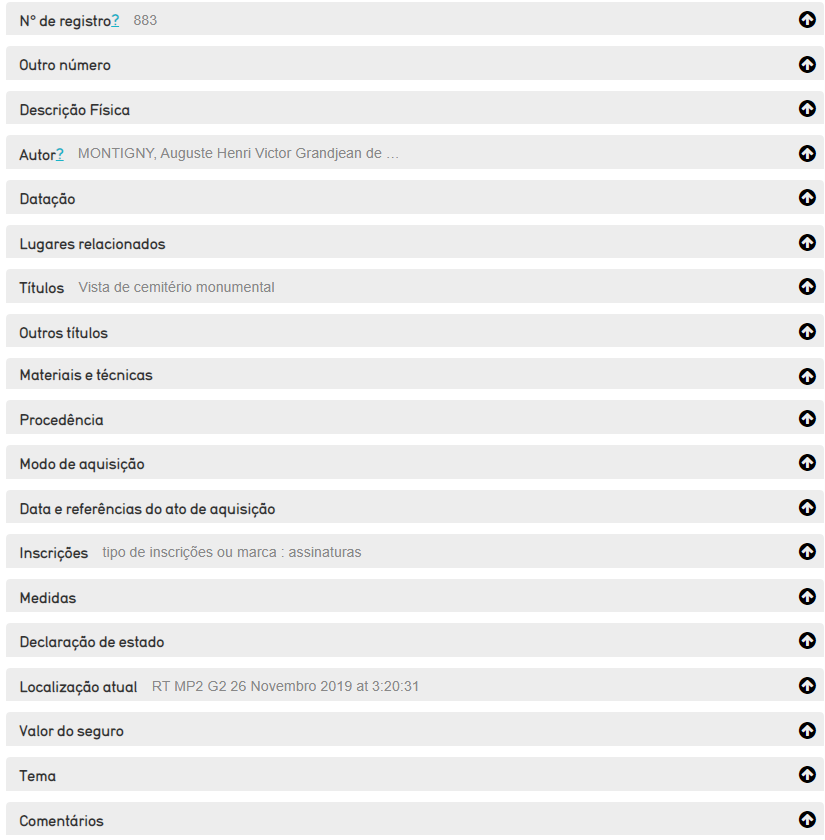
\includegraphics[width=\linewidth]{fichaId-01}
%	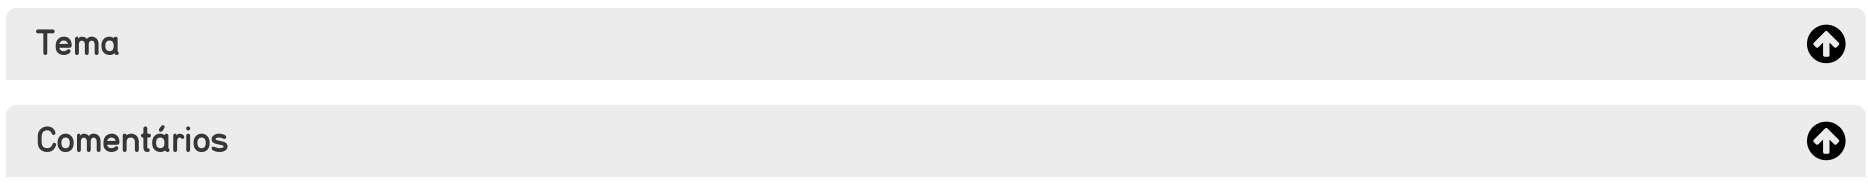
\includegraphics[width=\linewidth]{fichaId-02}
\end{flushleft}
%\begin{flushleft}
%	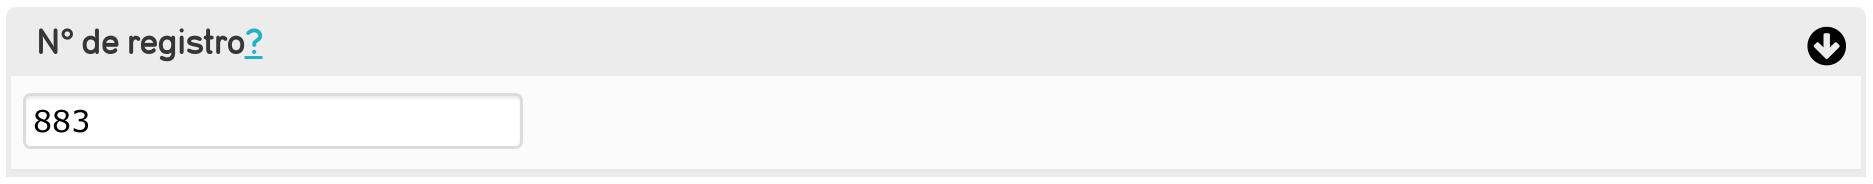
\includegraphics[width=\linewidth]{elemento-01}
%	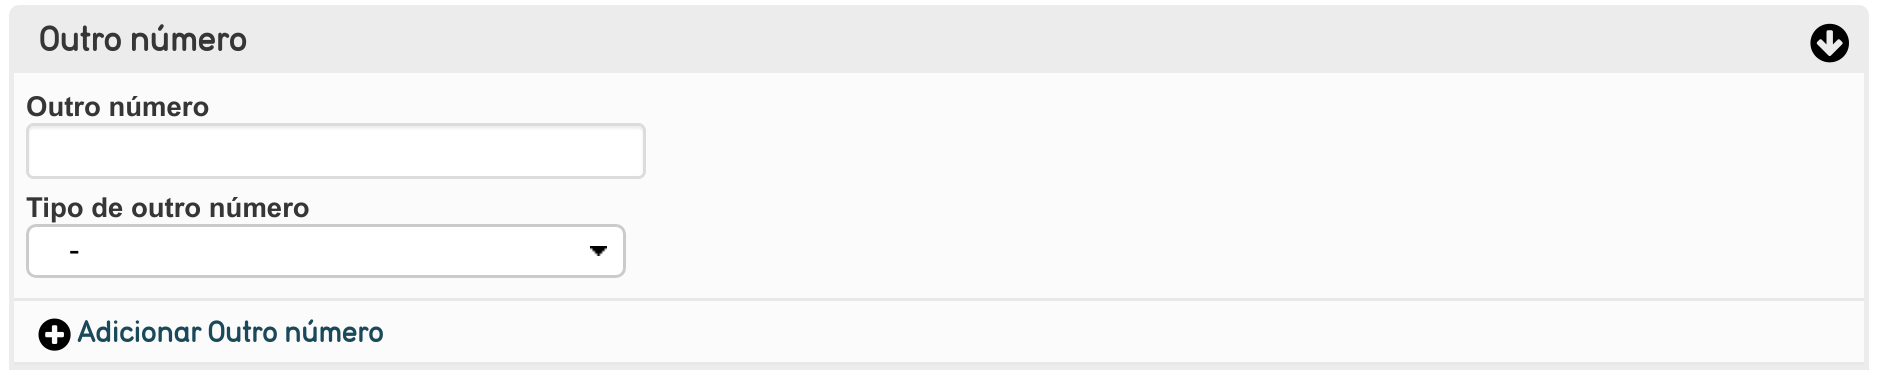
\includegraphics[width=\linewidth]{elemento-02}
%	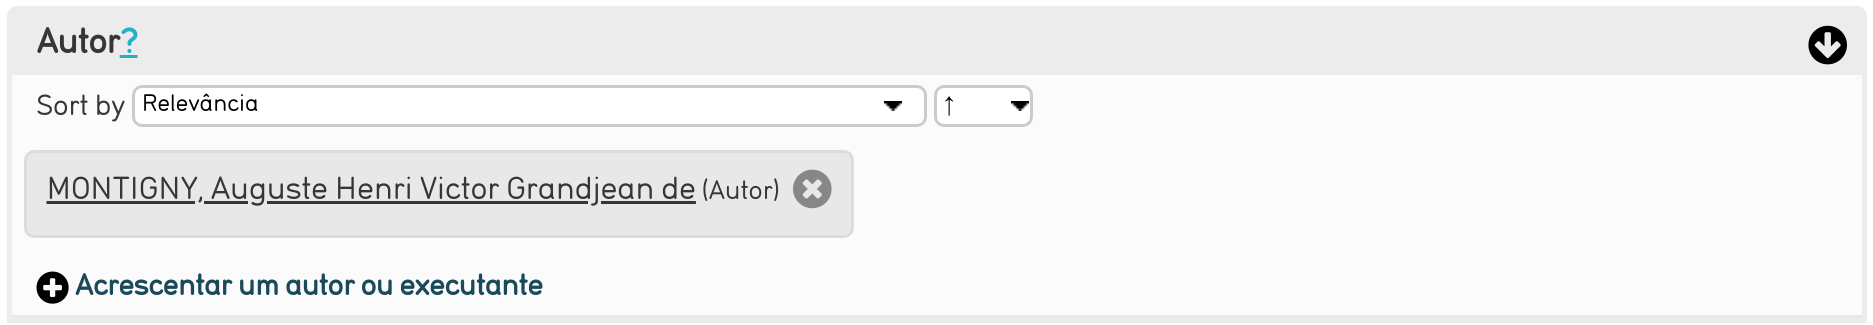
\includegraphics[width=\linewidth]{autor-01}
%	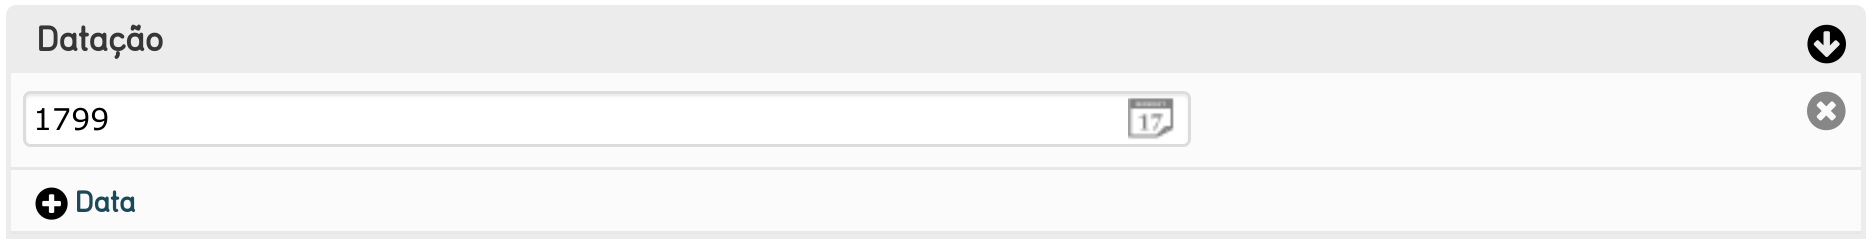
\includegraphics[width=\linewidth]{elemento-03}
%	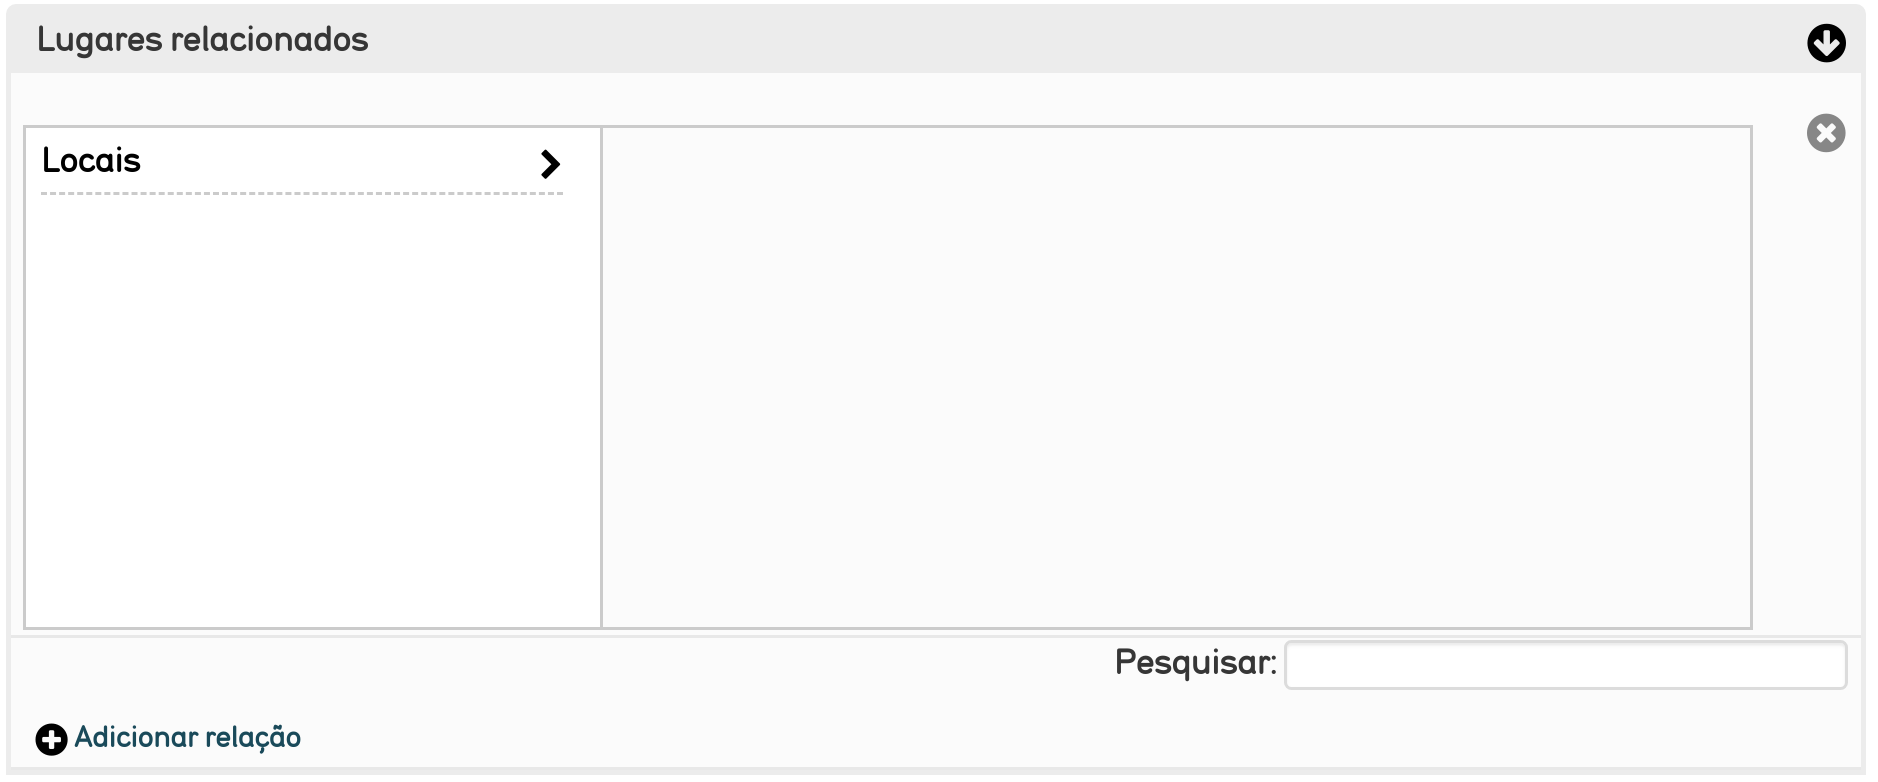
\includegraphics[width=\linewidth]{elemento-04}
%	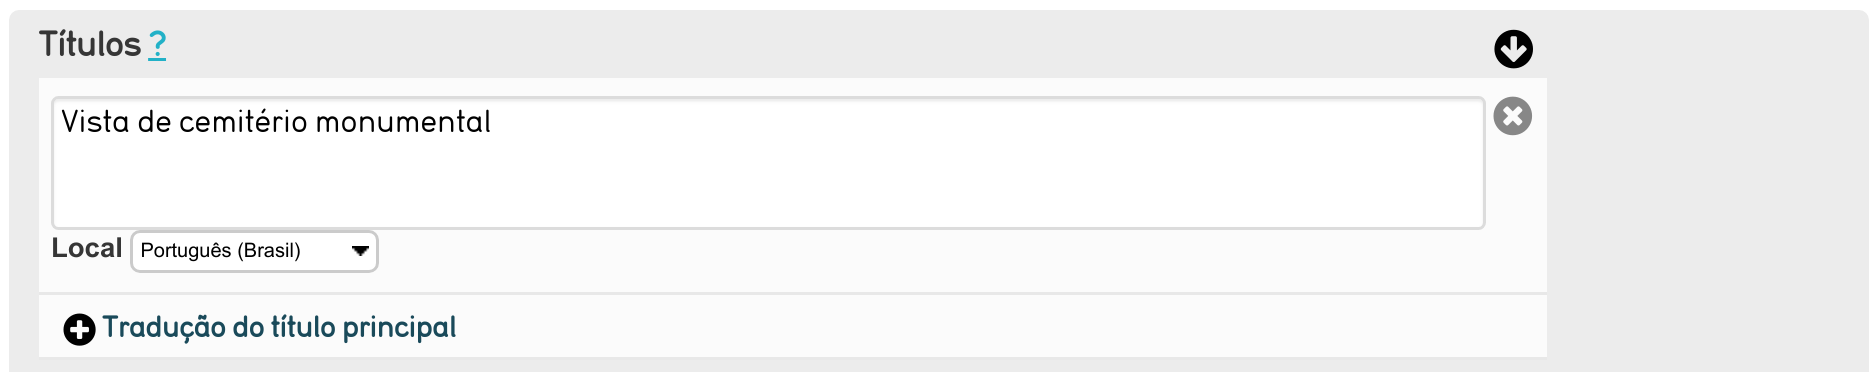
\includegraphics[width=\linewidth]{elemento-05}
%	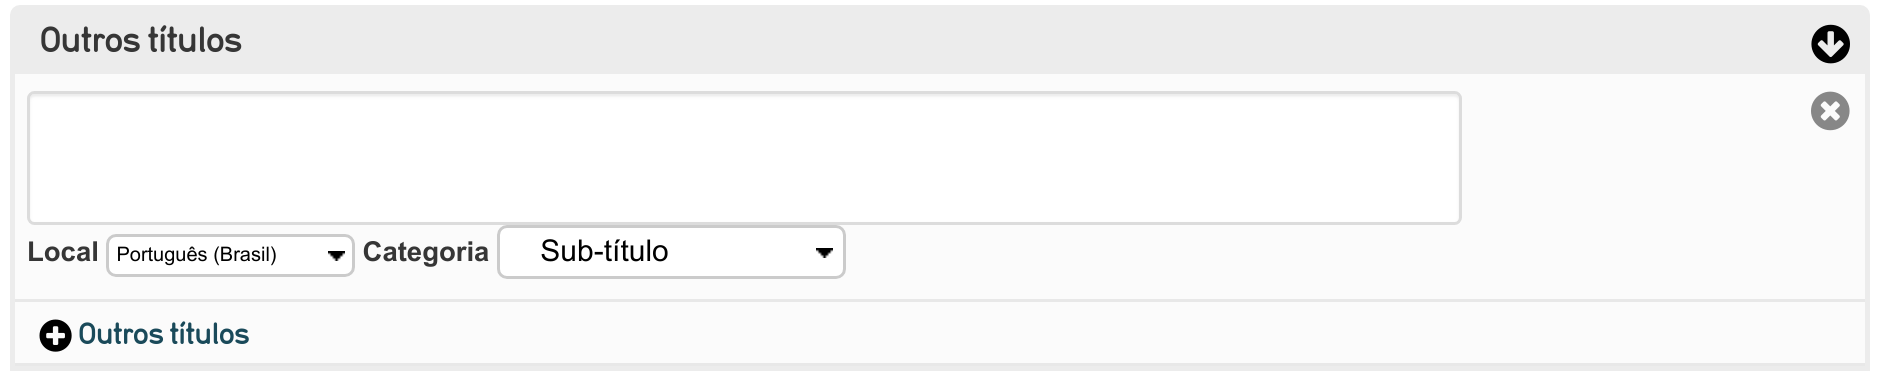
\includegraphics[width=\linewidth]{elemento-06}
%	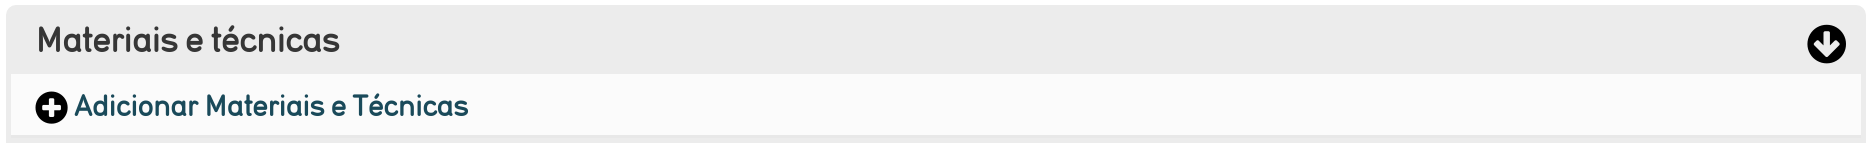
\includegraphics[width=\linewidth]{elemento-07}
%	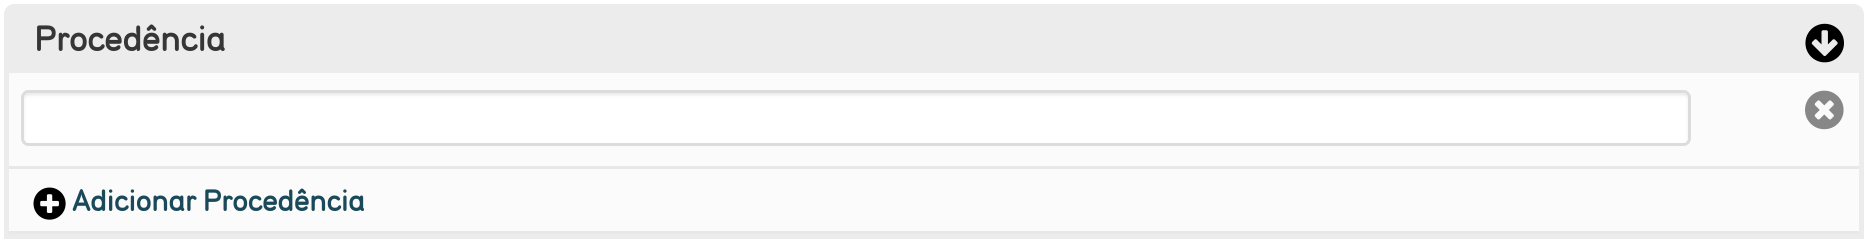
\includegraphics[width=\linewidth]{elemento-08}
%	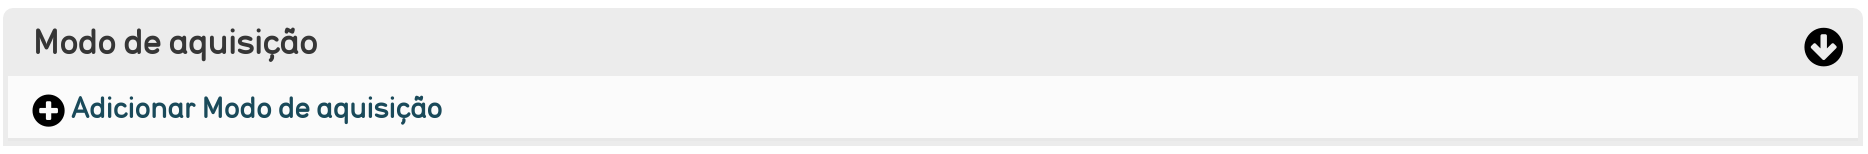
\includegraphics[width=\linewidth]{elemento-09}
%	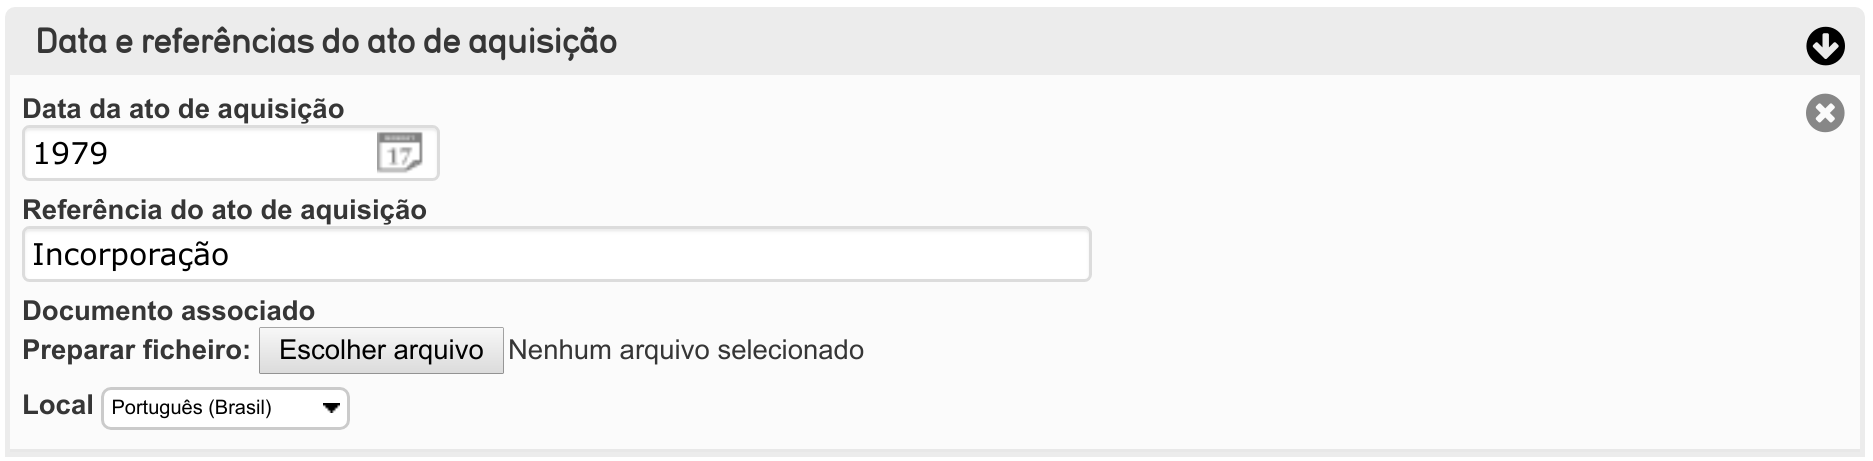
\includegraphics[width=\linewidth]{elemento-10}
%	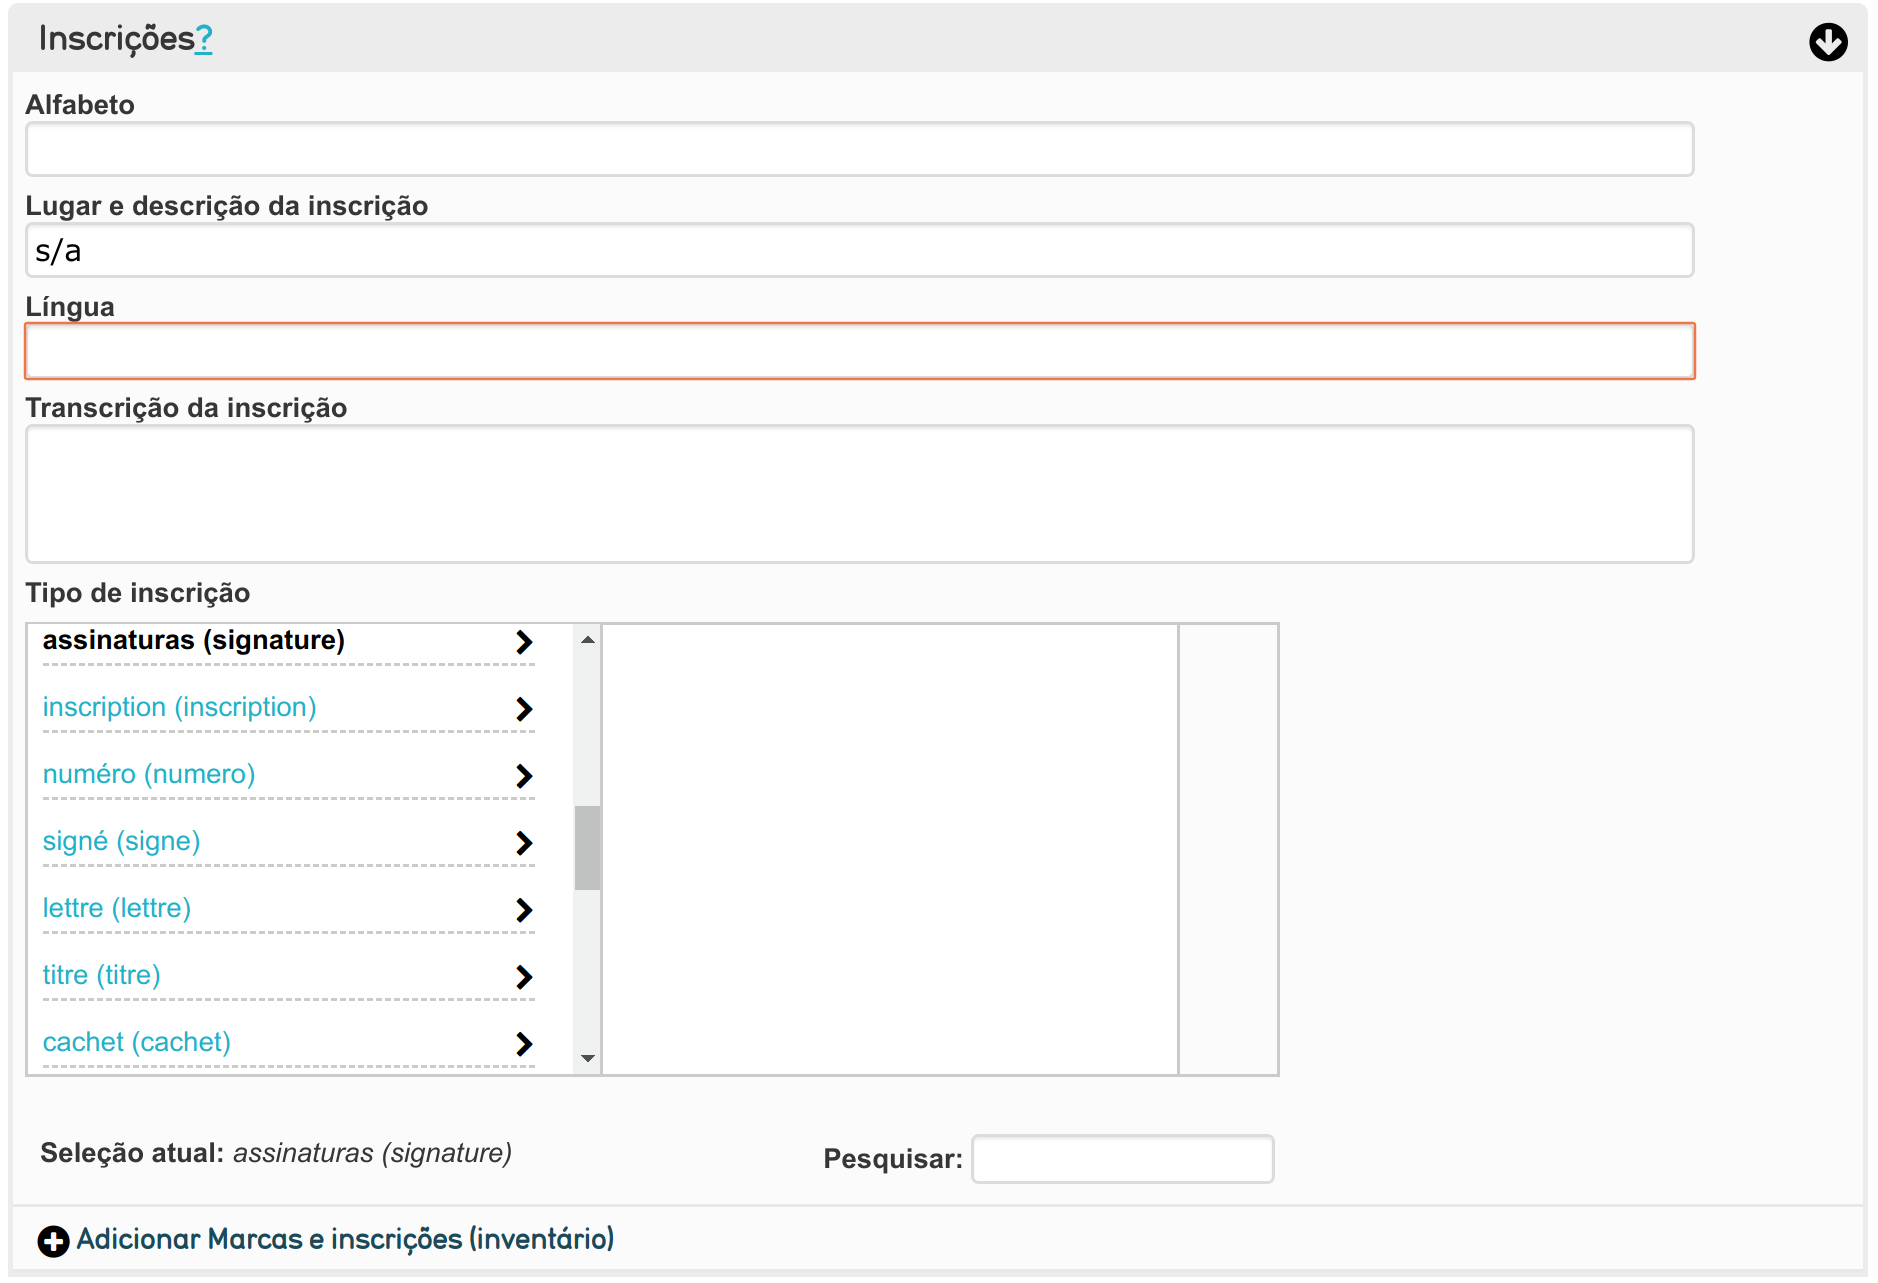
\includegraphics[width=\linewidth]{elemento-11}
%	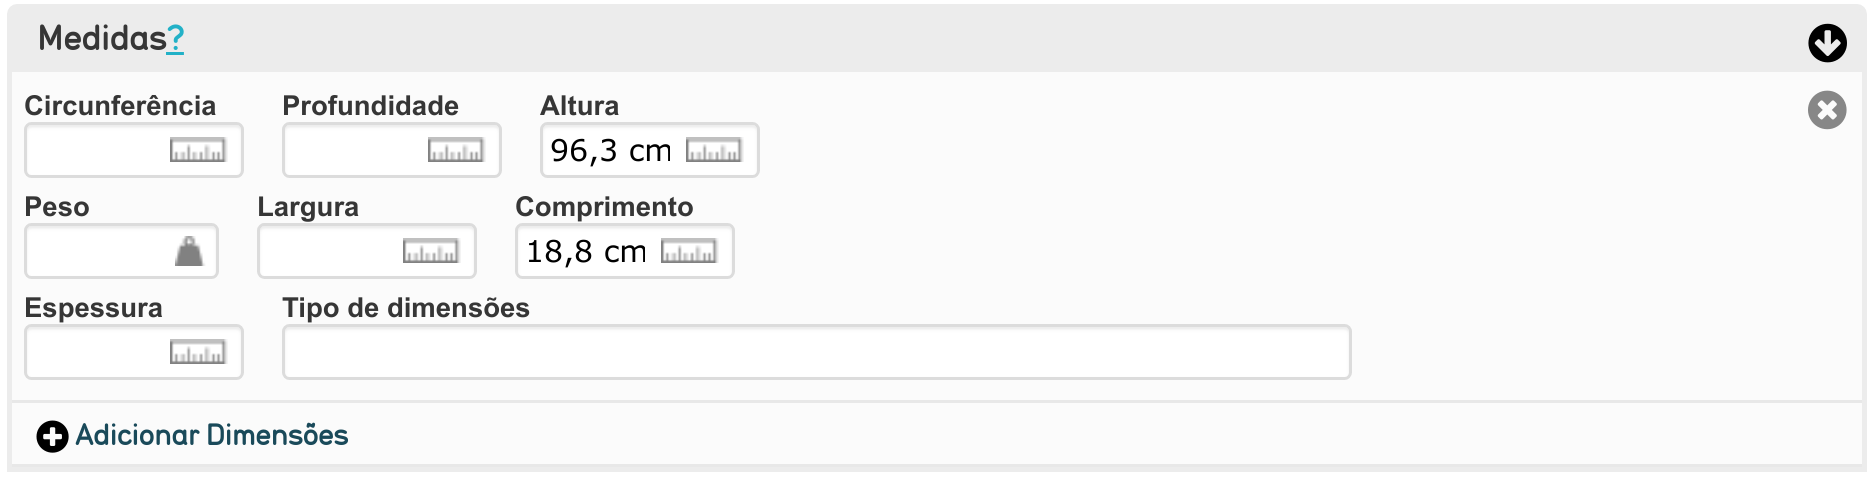
\includegraphics[width=\linewidth]{elemento-12}
%	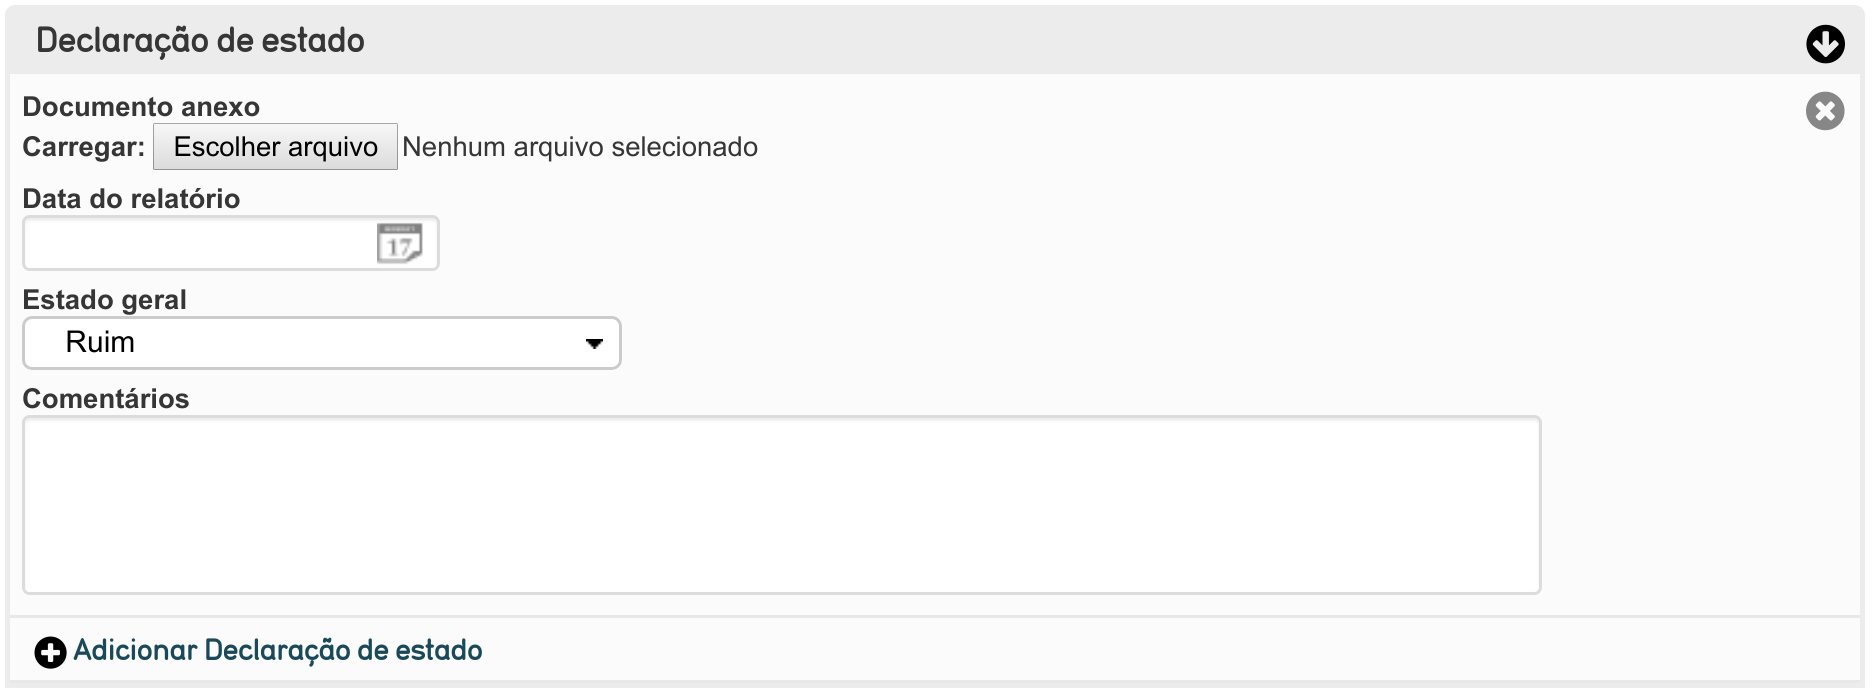
\includegraphics[width=\linewidth]{elemento-13}
%	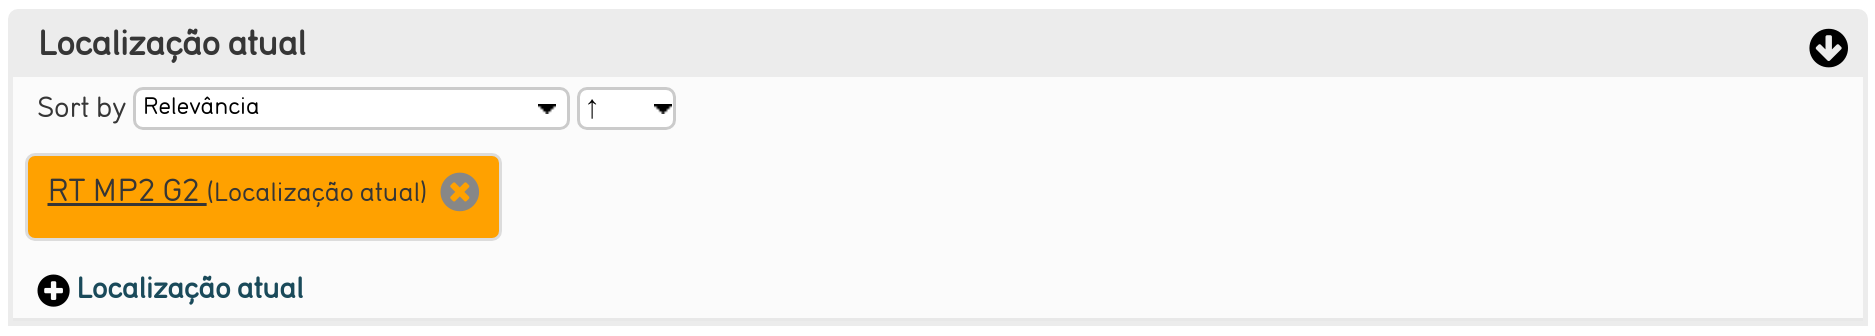
\includegraphics[width=\linewidth]{elemento-14}
%	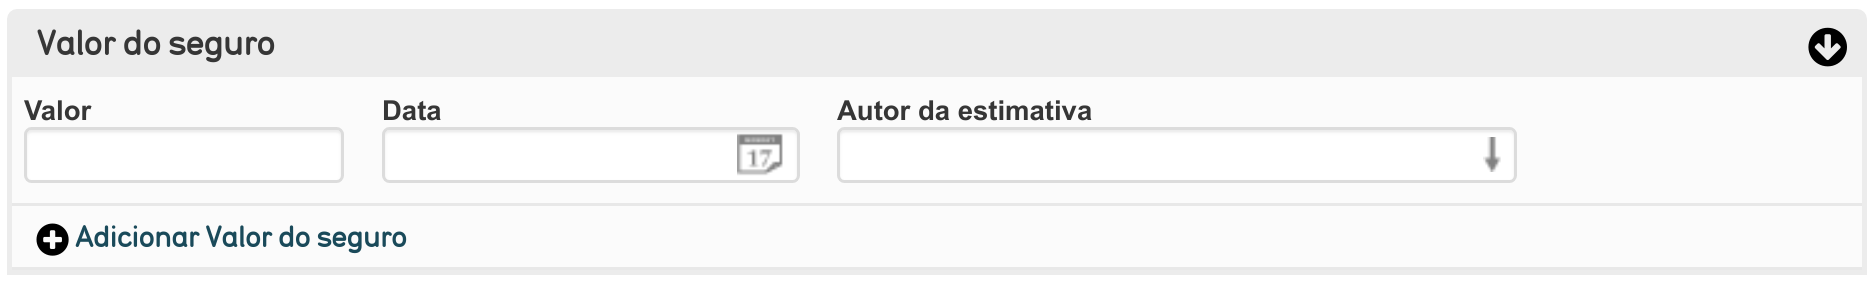
\includegraphics[width=\linewidth]{elemento-15}
%	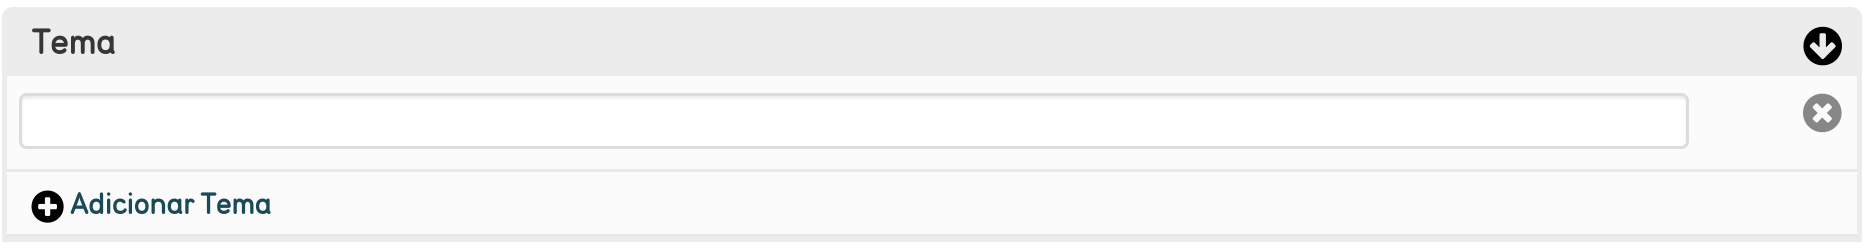
\includegraphics[width=\linewidth]{elemento-16}
%	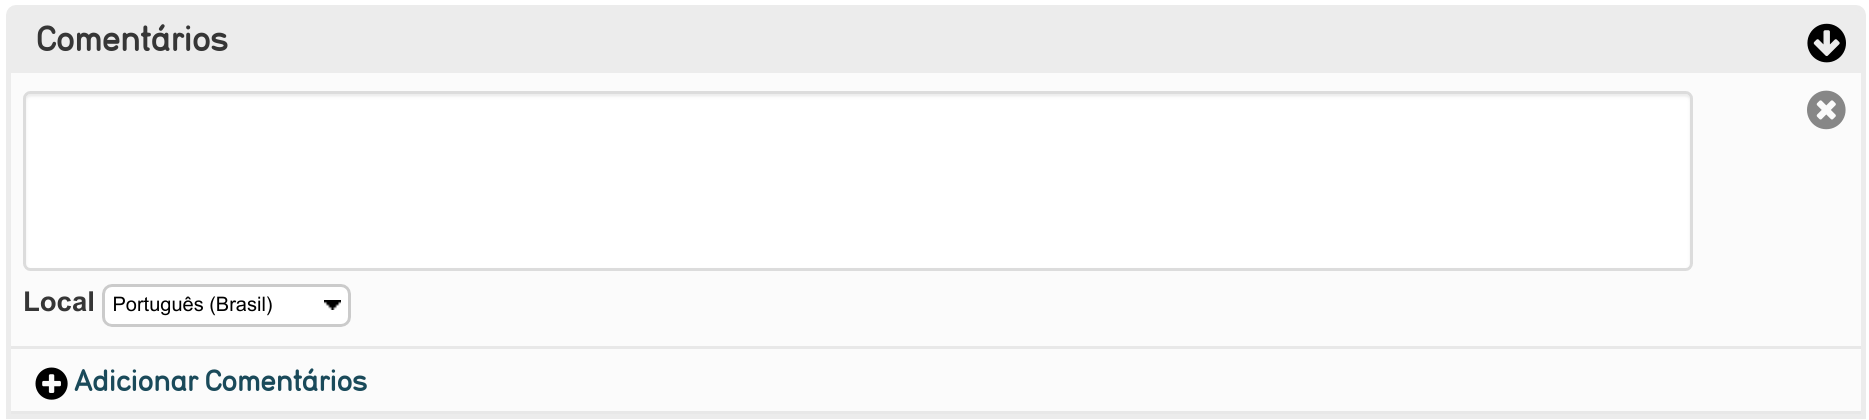
\includegraphics[width=\linewidth]{elemento-17}
%	
%\end{flushleft}
\subsection{Nº de registro}
\begin{flushleft}
	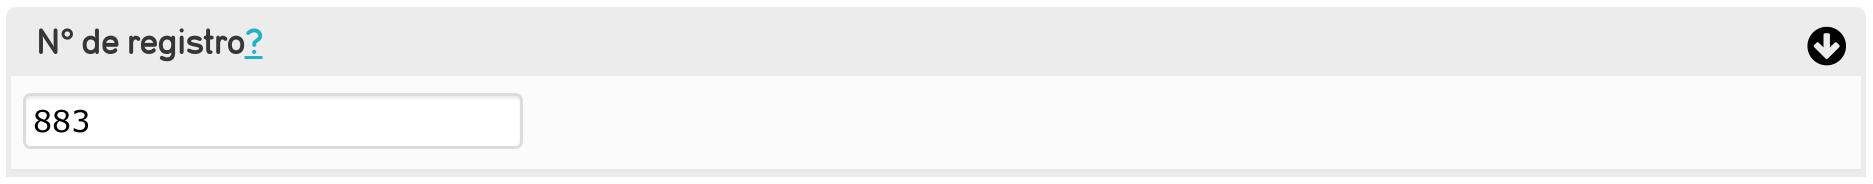
\includegraphics[width=\linewidth]{elemento-01}
\end{flushleft}
É o \textbf{número de registro de tombamento}. A numeração respeitou parcialmente o sistema numérico do Livro de Tombo encontrado, seguindo portanto, a sequência natural do número de ordem deste livro, cuja última peça fora registrada sob o número 2140. A primeira peça sem registro a ser inventariada recebeu, consequentemente, o número 2141.

Para tornar o sistema de numeração mais objetivo, optou-se por manter somente o número de ordem, abandonando o modelo tripartido do livro de tombo original, ou seja, omitindo-se os dígitos referentes ao ano de entrada da peça e a sua categoria. 

Para as peças compostas de diversas partes adotou-se o uso do complemento alfabético:

\begin{itemize}
	\item registro 1463 A - Classe Objetos Pessoais, Subclasse Objetos de adorno, Relógio - e 
	\item 1463 B - Classe Objetos pessoais, Subclasse Objetos de adorno, Estojo.
\end{itemize}

\subsection{Outro número}
\begin{flushleft}
	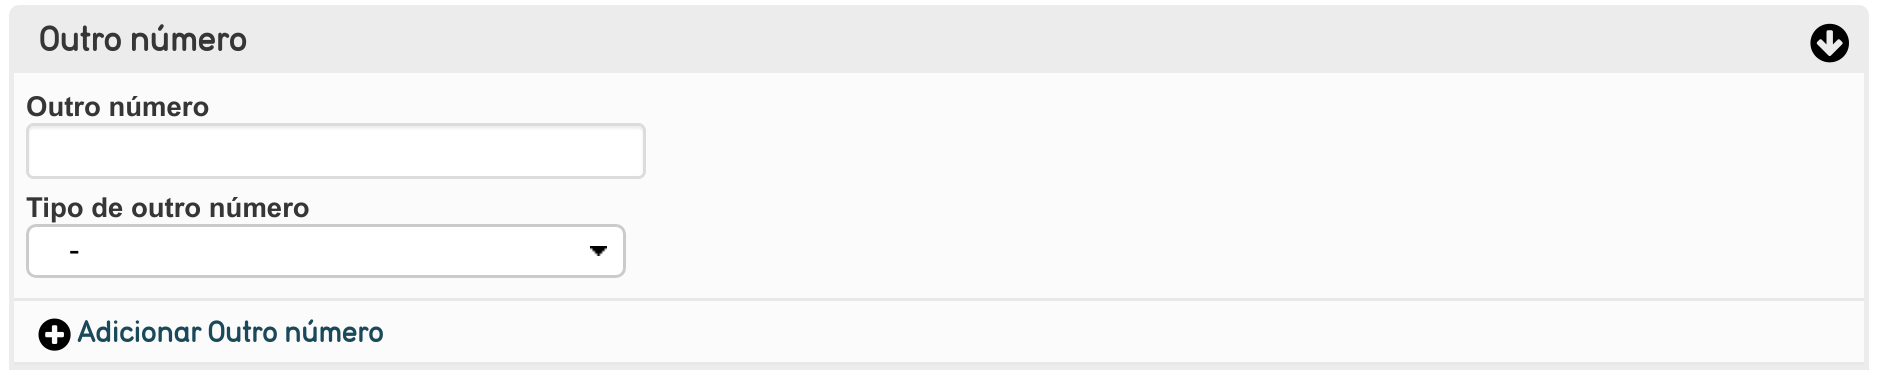
\includegraphics[width=\linewidth]{elemento-02}
\end{flushleft}
Alguma outra referência para o objeto. O tipo de número também pode ser especificado:
\begin{itemize}
	\item Antigo número do inventário
	\item Ficha do museu
	\item Número antigo
	\item Número de classificação
	\item Número de inventário na coleção do depositante
	\item Número dentro da coleção do proprietário
	\item Número de verificação
	\item Número no Registro da UFRJ
\end{itemize}
\begin{flushleft}
	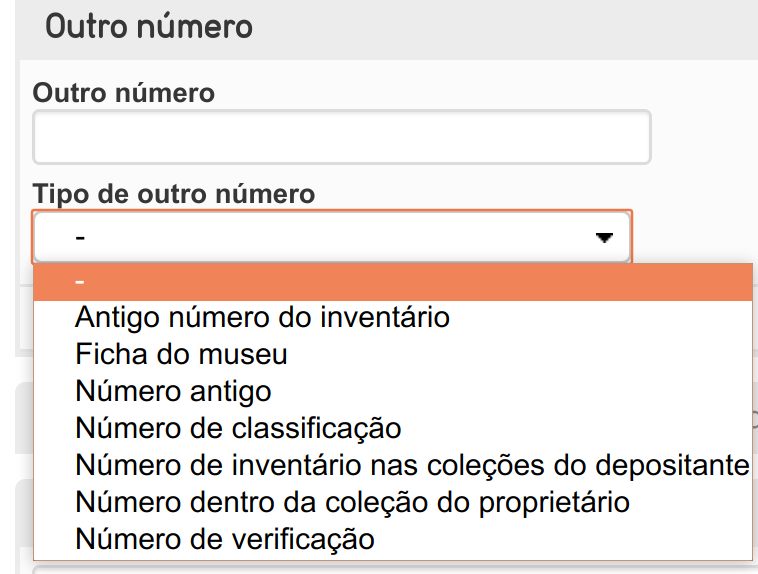
\includegraphics[width=0.5\linewidth]{tipoOutroNumero}
\end{flushleft}

\subsection{Descrição Física}

\begin{flushleft}
	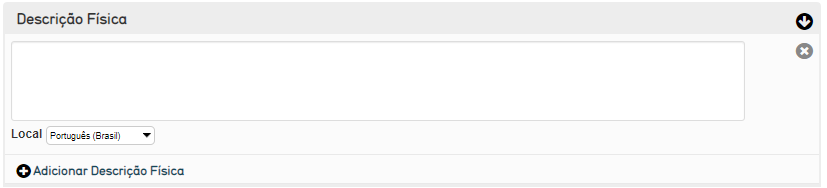
\includegraphics[width=\linewidth]{DescricFisica}
\end{flushleft}

Campo destinado à escrita livre sobre a descrição física do objeto.

\subsection{Autor}
\begin{flushleft}
	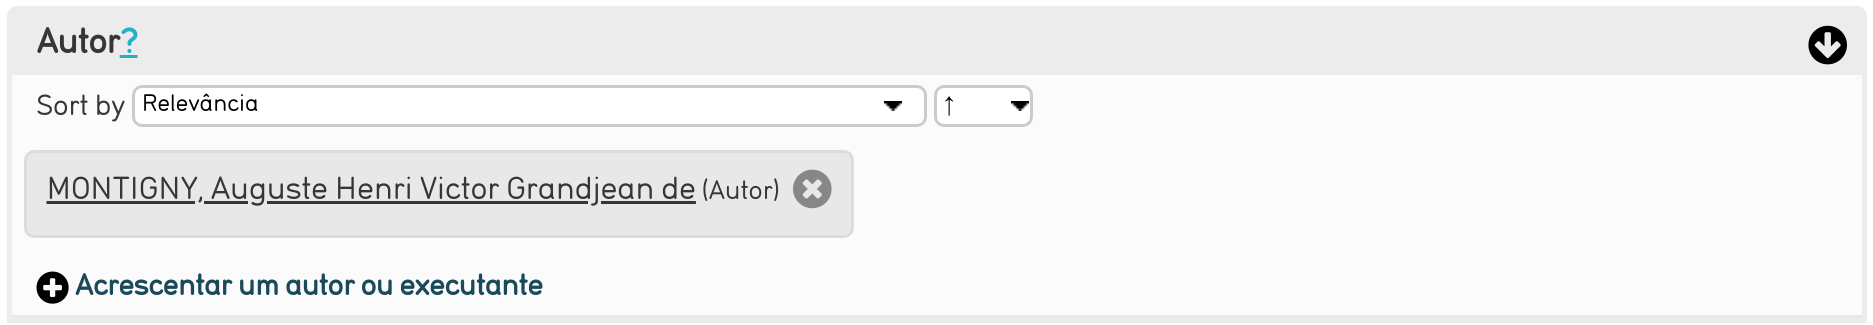
\includegraphics[width=\linewidth]{autor-01}
\end{flushleft}
Campo destinado ao registro de pessoa física ou jurídica que concebeu material e/ou intelectualmente a obra. Podem ser acrescentados outros autores.

\subsection{Datação}
\begin{flushleft}
	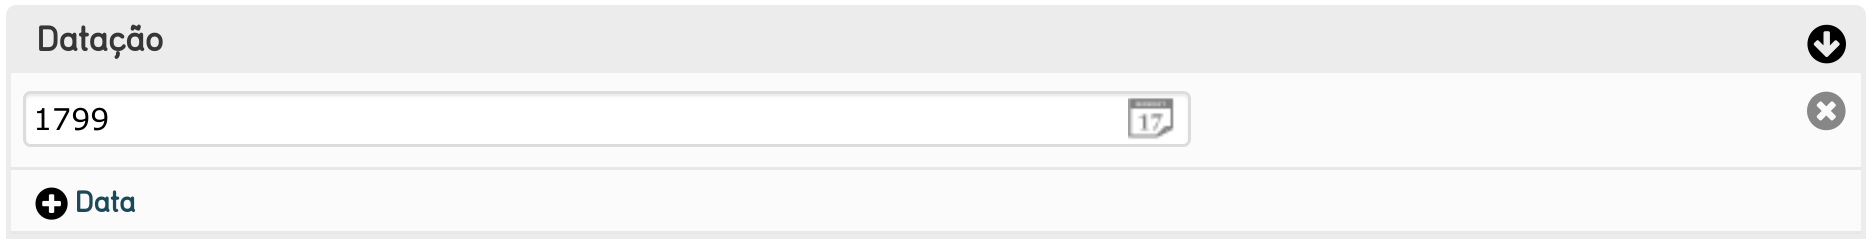
\includegraphics[width=\linewidth]{elemento-03}
\end{flushleft}

\subsection{Lugares relacionados}
\begin{flushleft}
	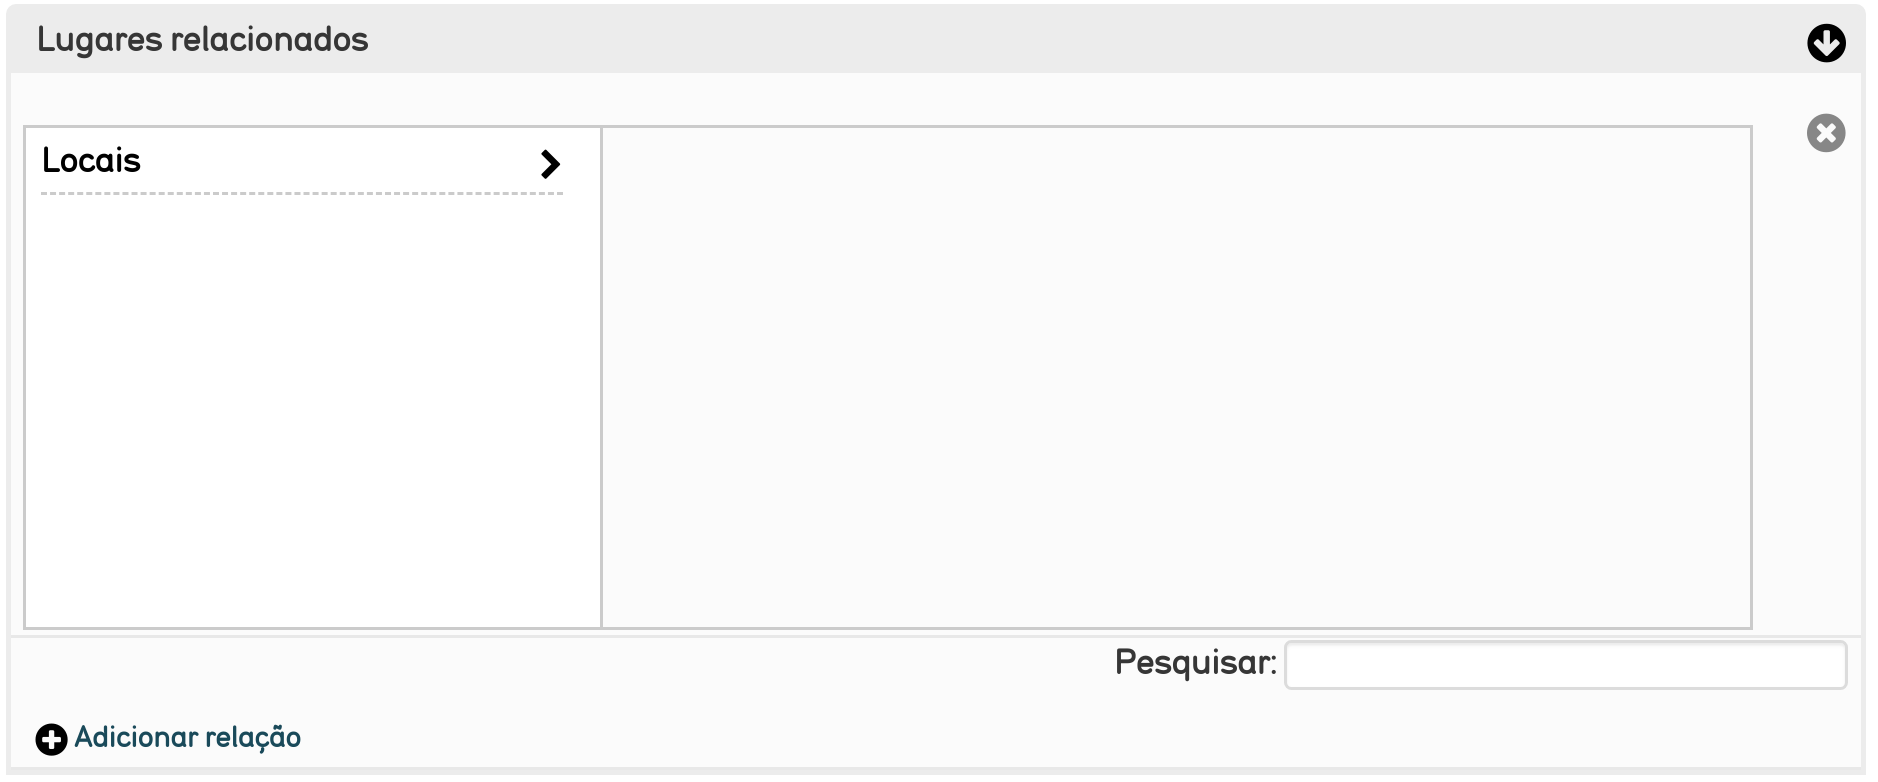
\includegraphics[width=\linewidth]{elemento-04}
\end{flushleft}

Além do lugar relacionado também se deve escolher a relação do lugar com a obra por meio do menu disponível.

\begin{flushleft}
	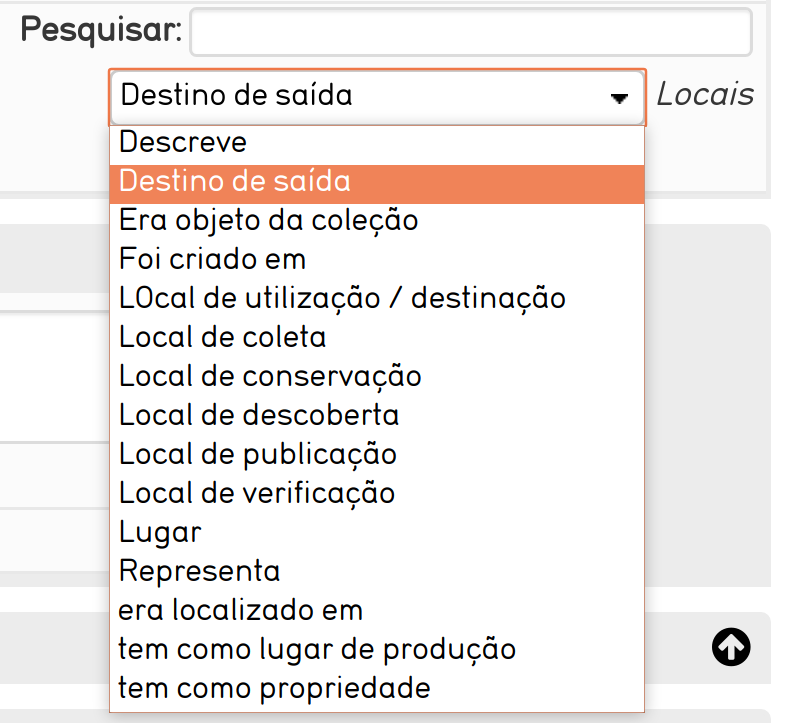
\includegraphics[width=0.5\linewidth]{descreveLugar}
\end{flushleft}

\subsection{Títulos}
\begin{flushleft}
	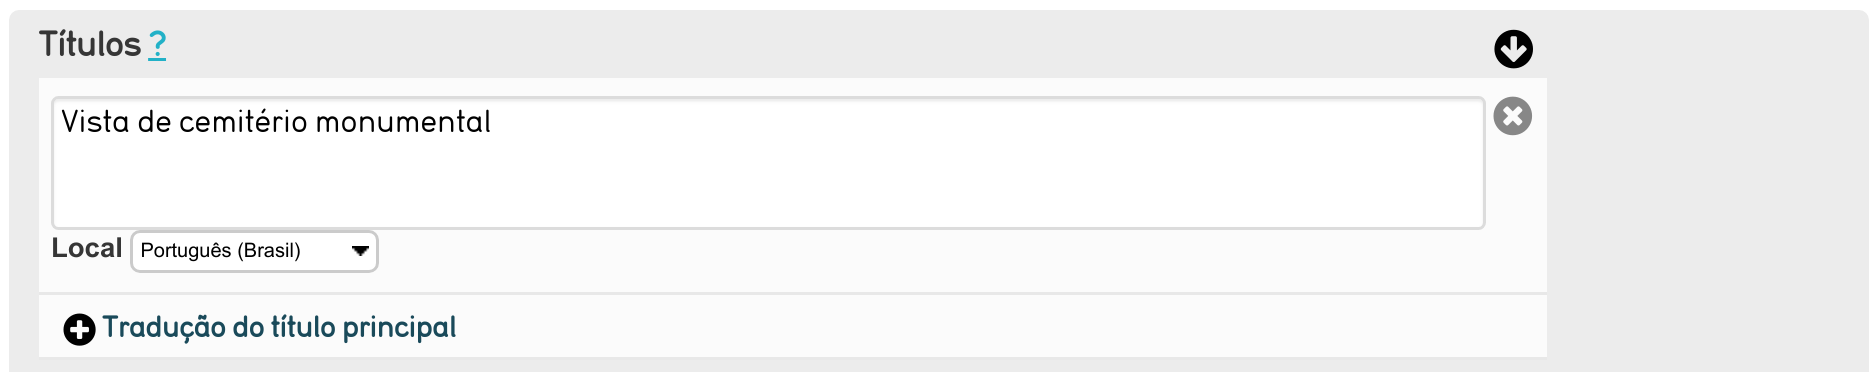
\includegraphics[width=\linewidth]{elemento-05}
\end{flushleft}
Também é possível fornecer uma tradução em outras línguas do título da obra.

\subsection{Outros títulos}
\begin{flushleft}
	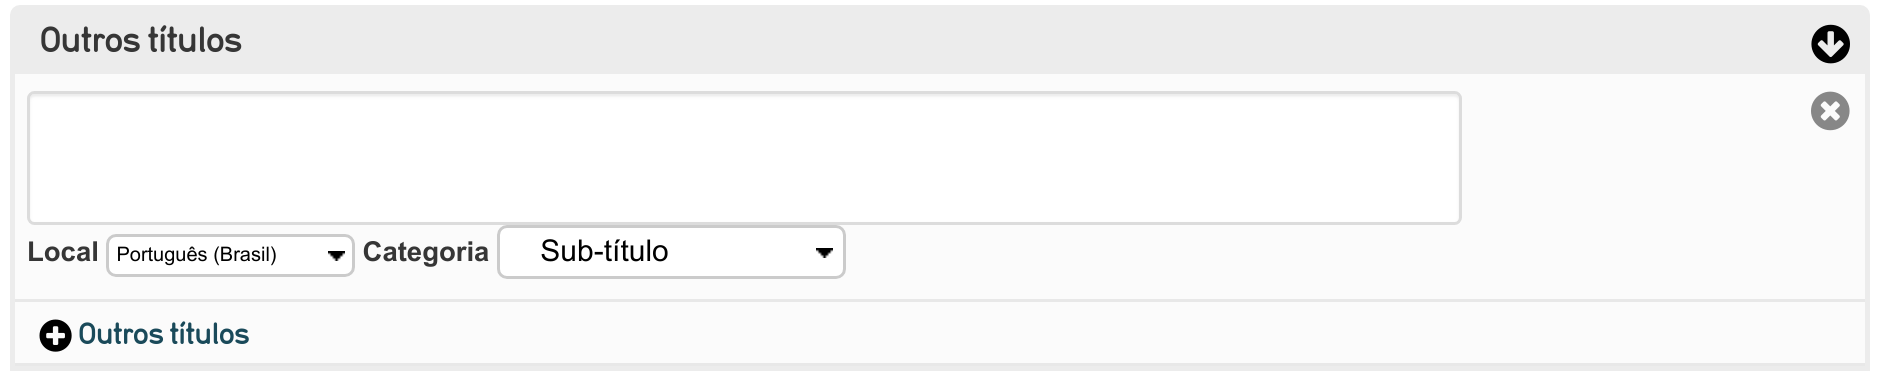
\includegraphics[width=\linewidth]{elemento-06}
\end{flushleft}

\subsection{Materiais e técnicas}
\begin{flushleft}
	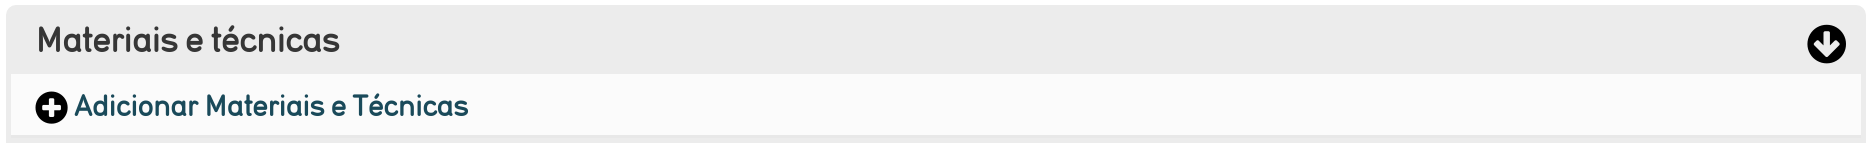
\includegraphics[width=\linewidth]{elemento-07}
\end{flushleft}

\subsection{Procedência}
\begin{flushleft}
	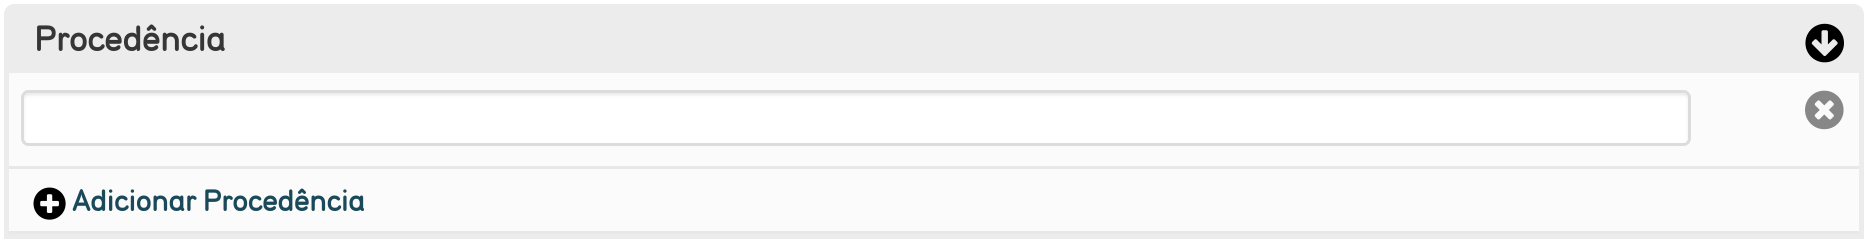
\includegraphics[width=\linewidth]{elemento-08}
\end{flushleft}

\subsection{Modo de aquisição}
\begin{flushleft}
	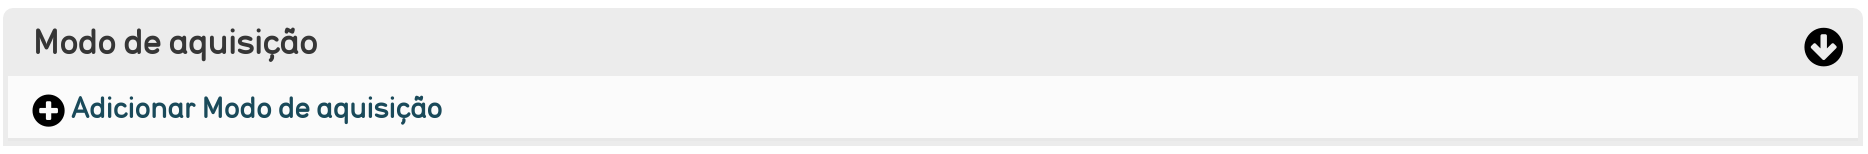
\includegraphics[width=\linewidth]{elemento-09}
\end{flushleft}

\subsection{Data e referências so ato de aquisição}
\begin{flushleft}
	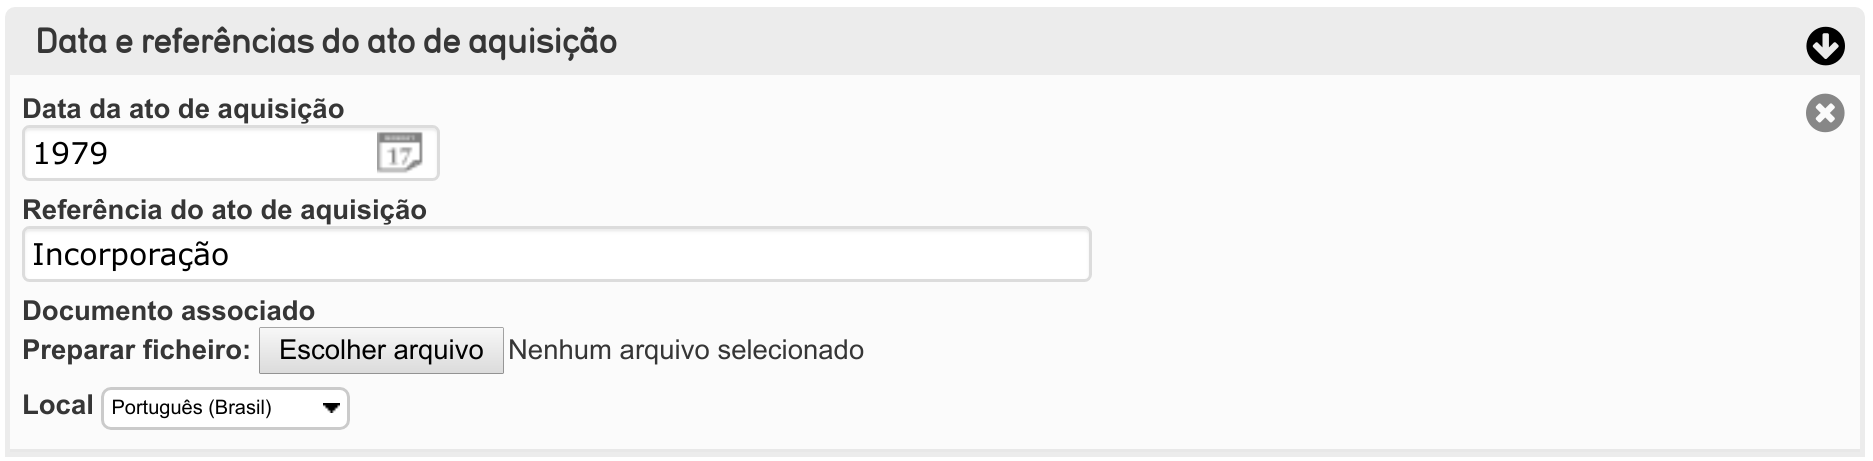
\includegraphics[width=\linewidth]{elemento-10}
\end{flushleft}

\subsection{Inscrições}
\begin{flushleft}
	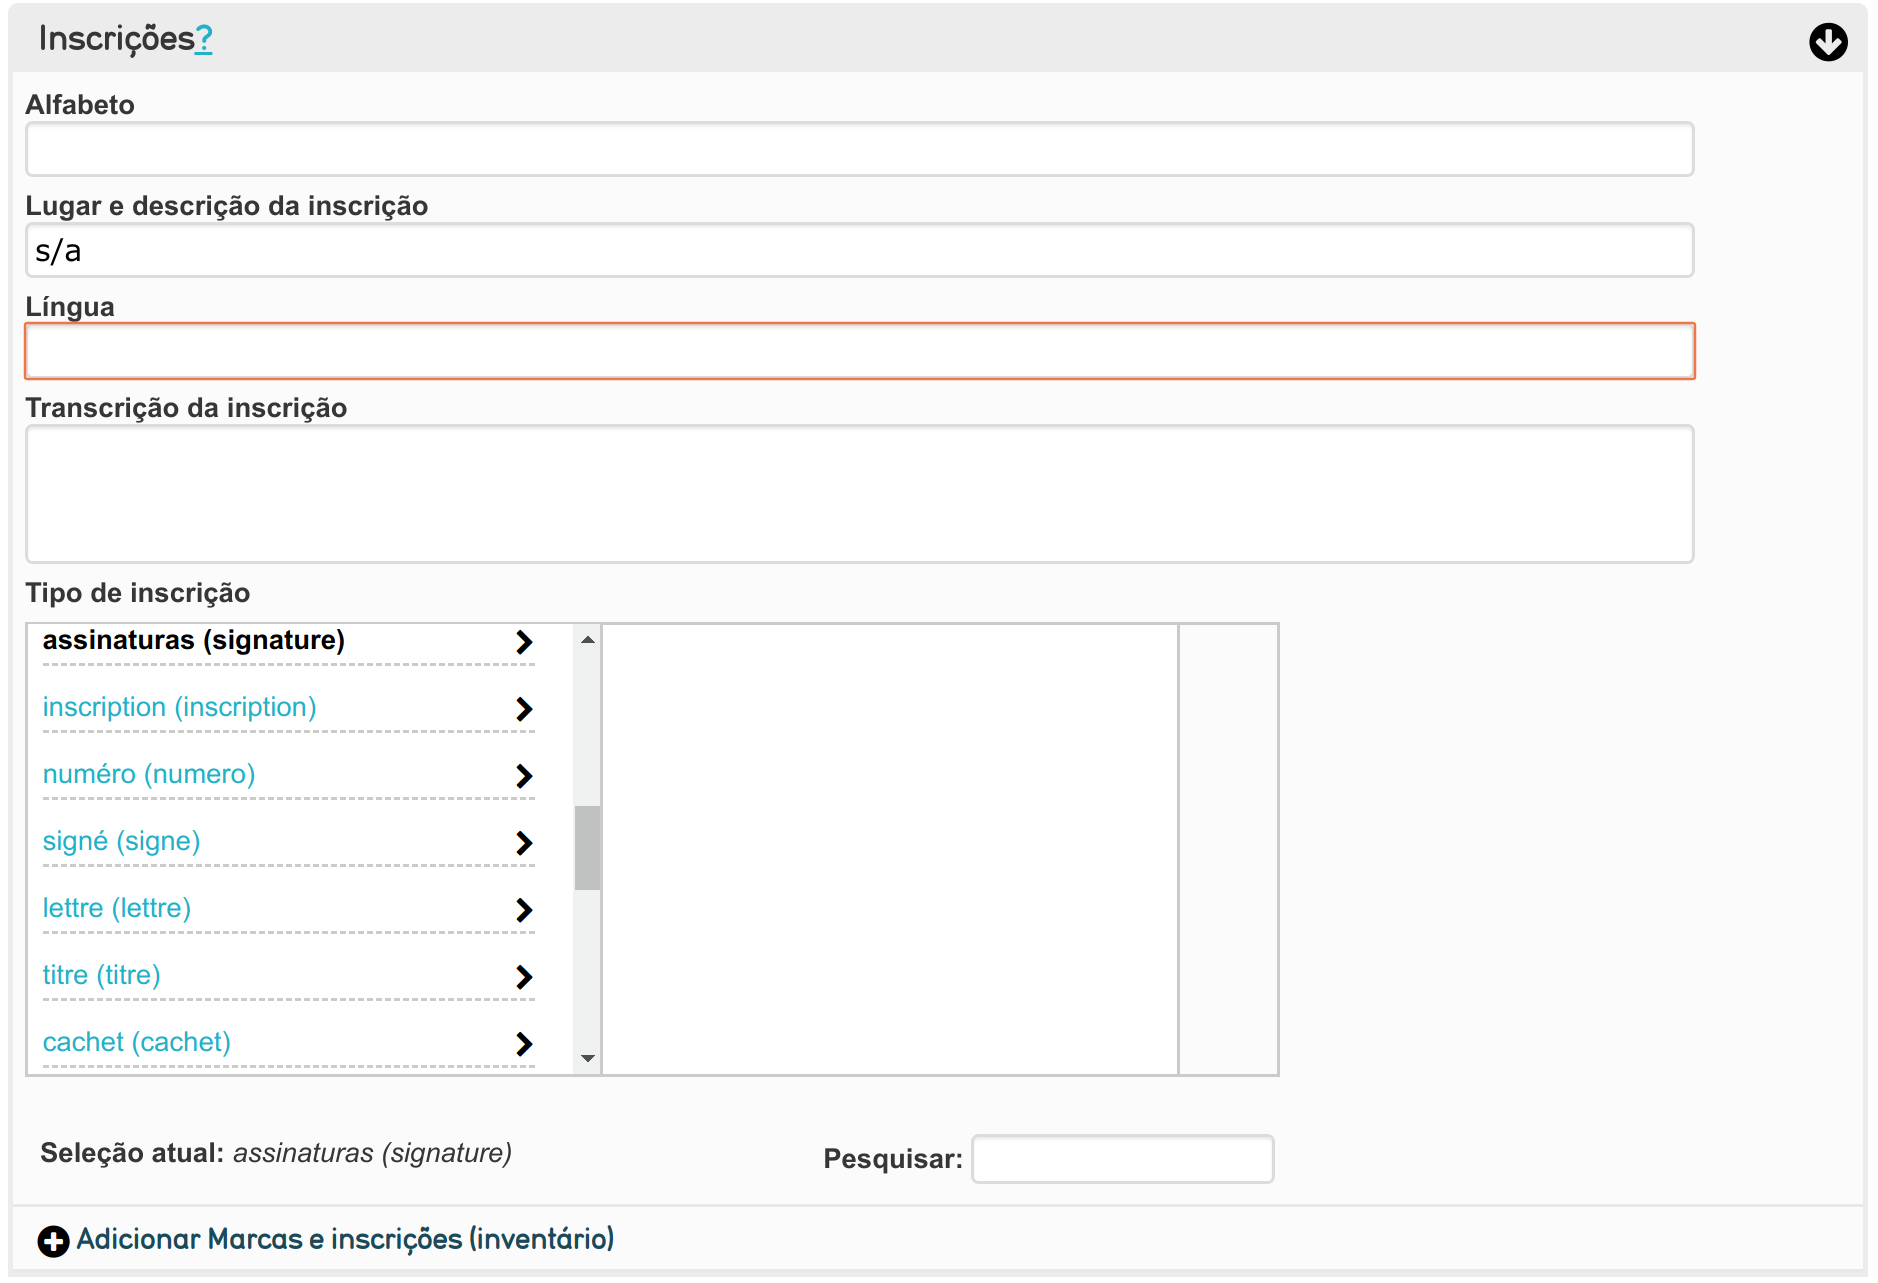
\includegraphics[width=\linewidth]{elemento-11}
\end{flushleft}

\subsection{Medidas}
\begin{flushleft}
	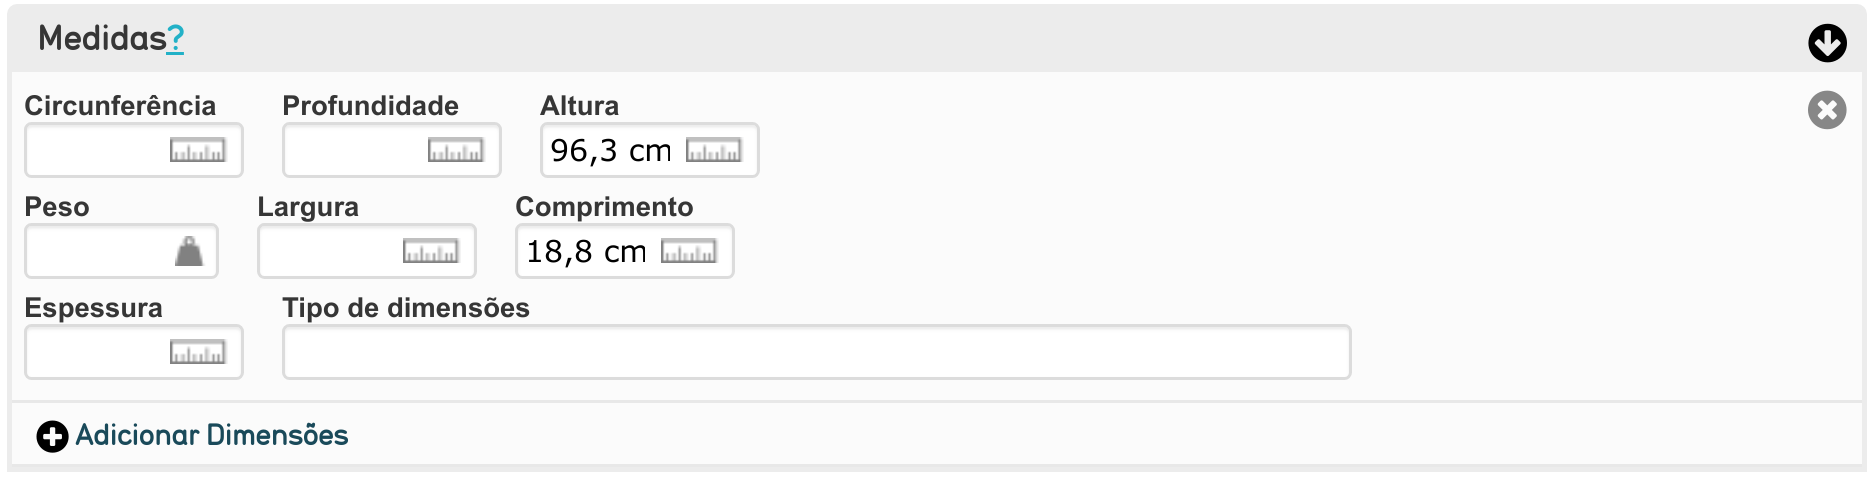
\includegraphics[width=\linewidth]{elemento-12}
\end{flushleft}

\subsection{Declaração de estado}
\begin{flushleft}
	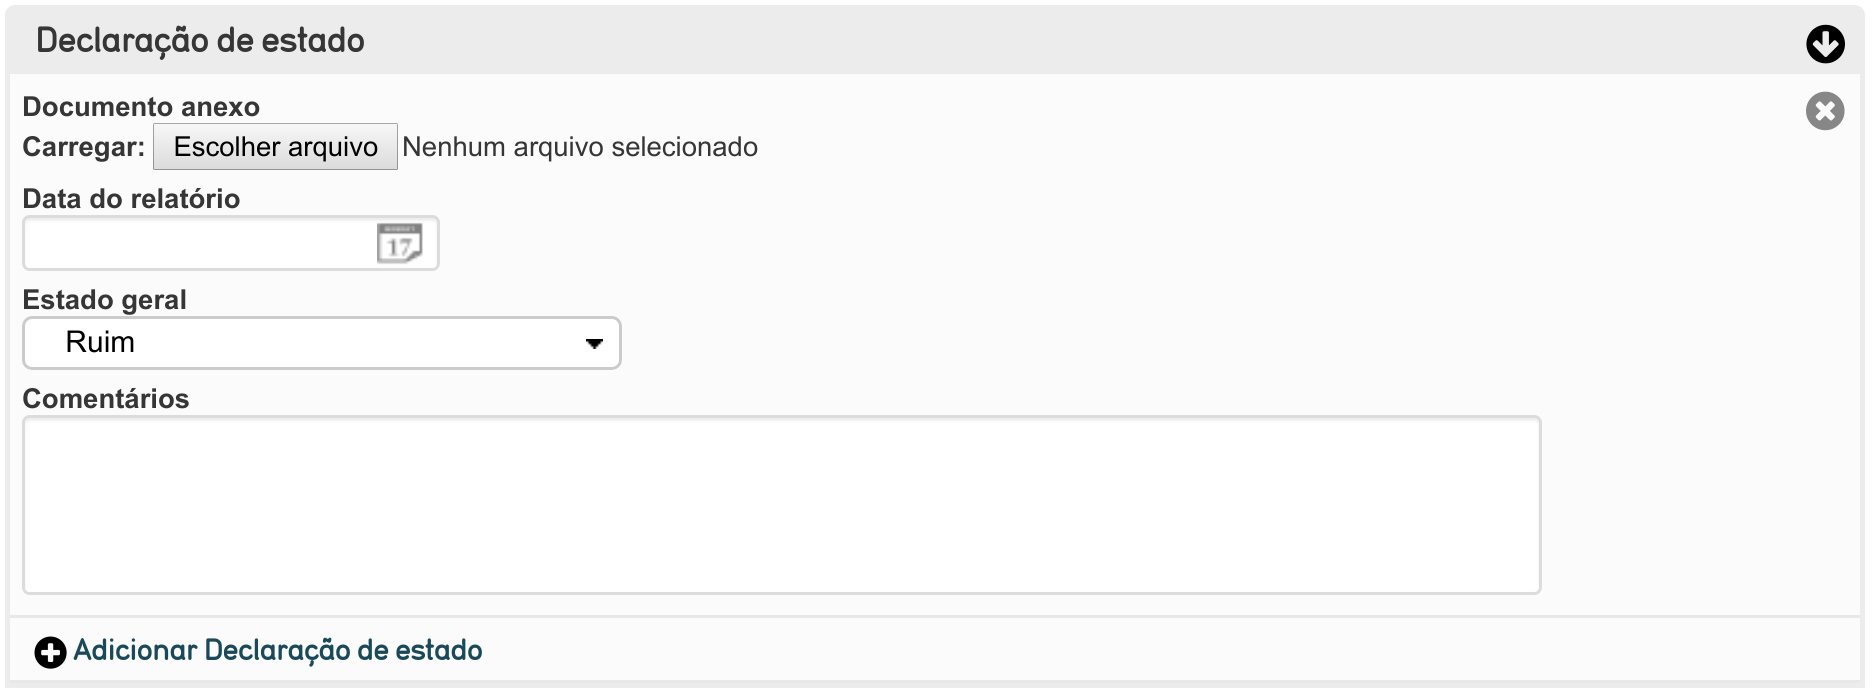
\includegraphics[width=\linewidth]{elemento-13}
\end{flushleft}

\subsection{Localização atual}
\begin{flushleft}
	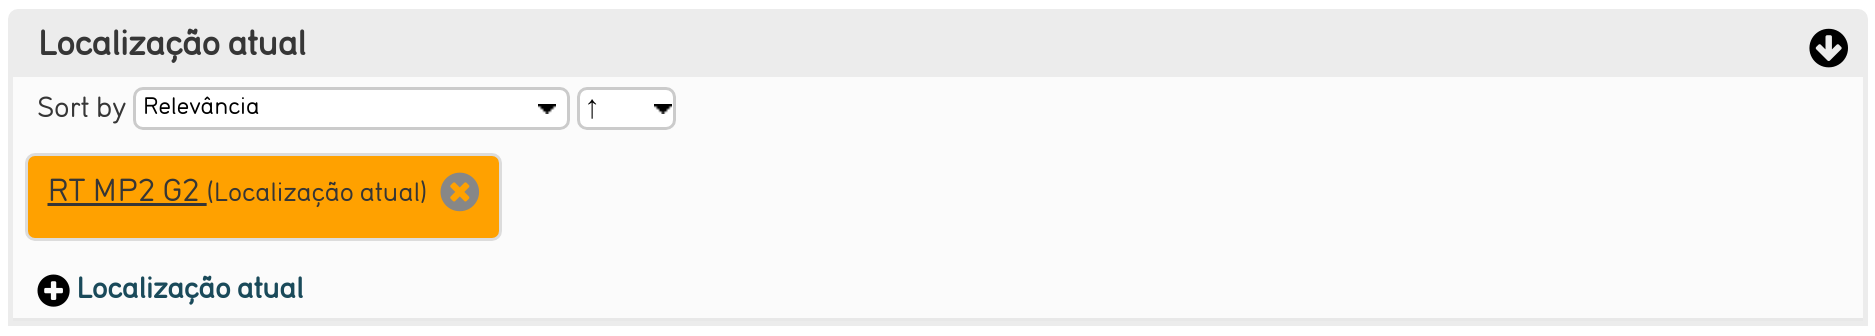
\includegraphics[width=\linewidth]{elemento-14}
\end{flushleft}

\subsection{Valor do seguro}
\begin{flushleft}
	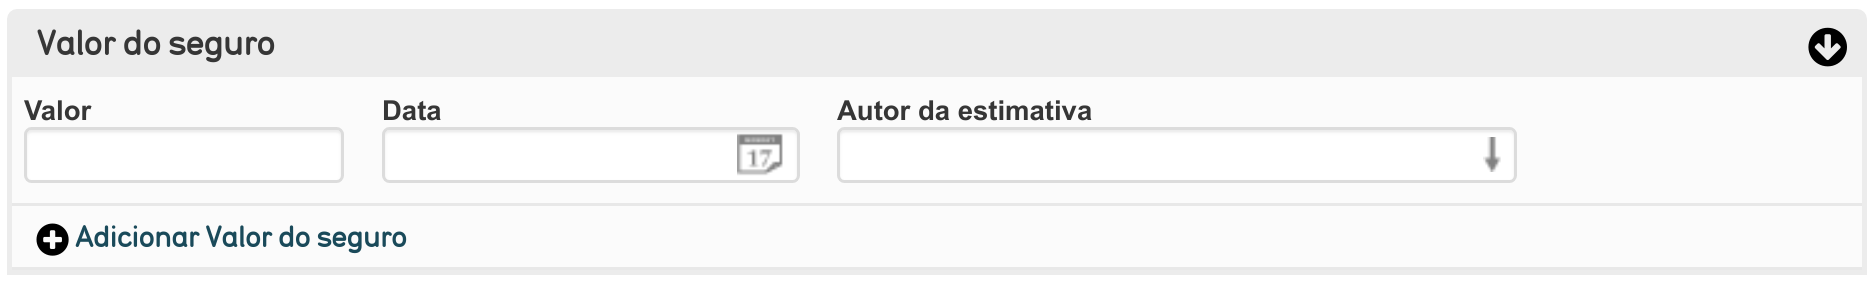
\includegraphics[width=\linewidth]{elemento-15}
\end{flushleft}

\subsection{Tema}
\begin{flushleft}
	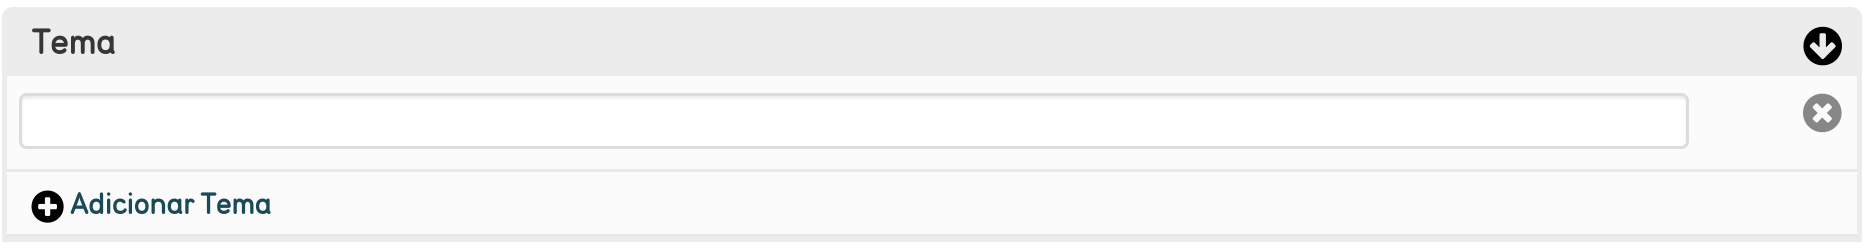
\includegraphics[width=\linewidth]{elemento-16}
\end{flushleft}

\subsection{Comentários}
\begin{flushleft}
	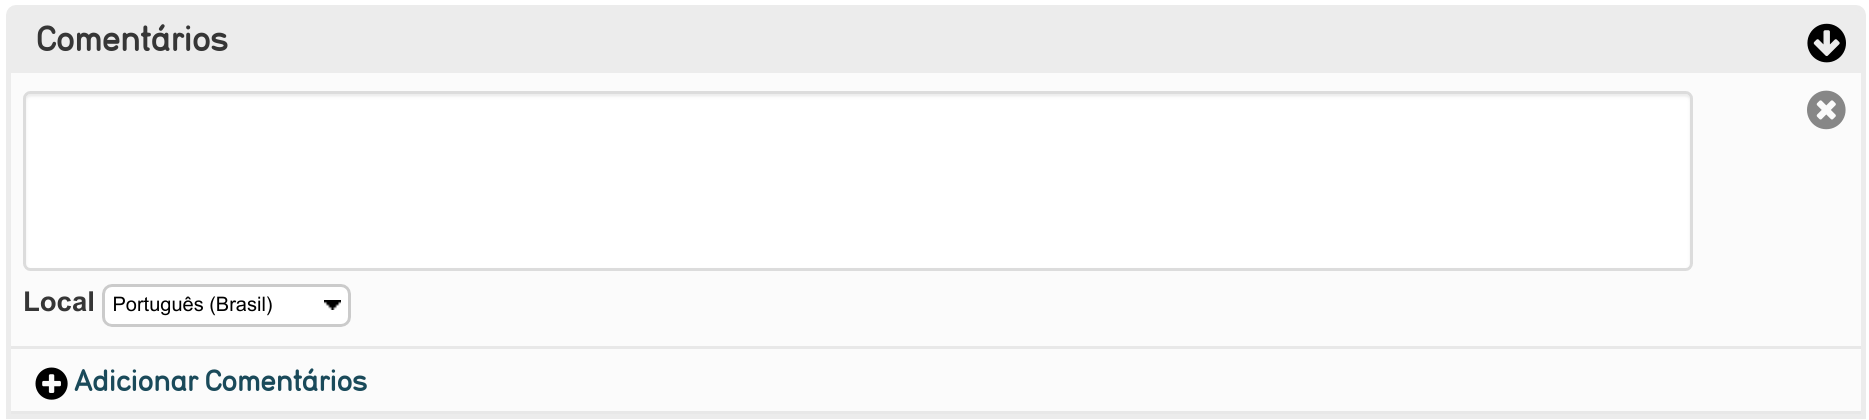
\includegraphics[width=\linewidth]{elemento-17}
\end{flushleft}

\section{Ficha Análise Histórica e Estilística}
\subsection{Visão Geral}
\begin{flushleft}
	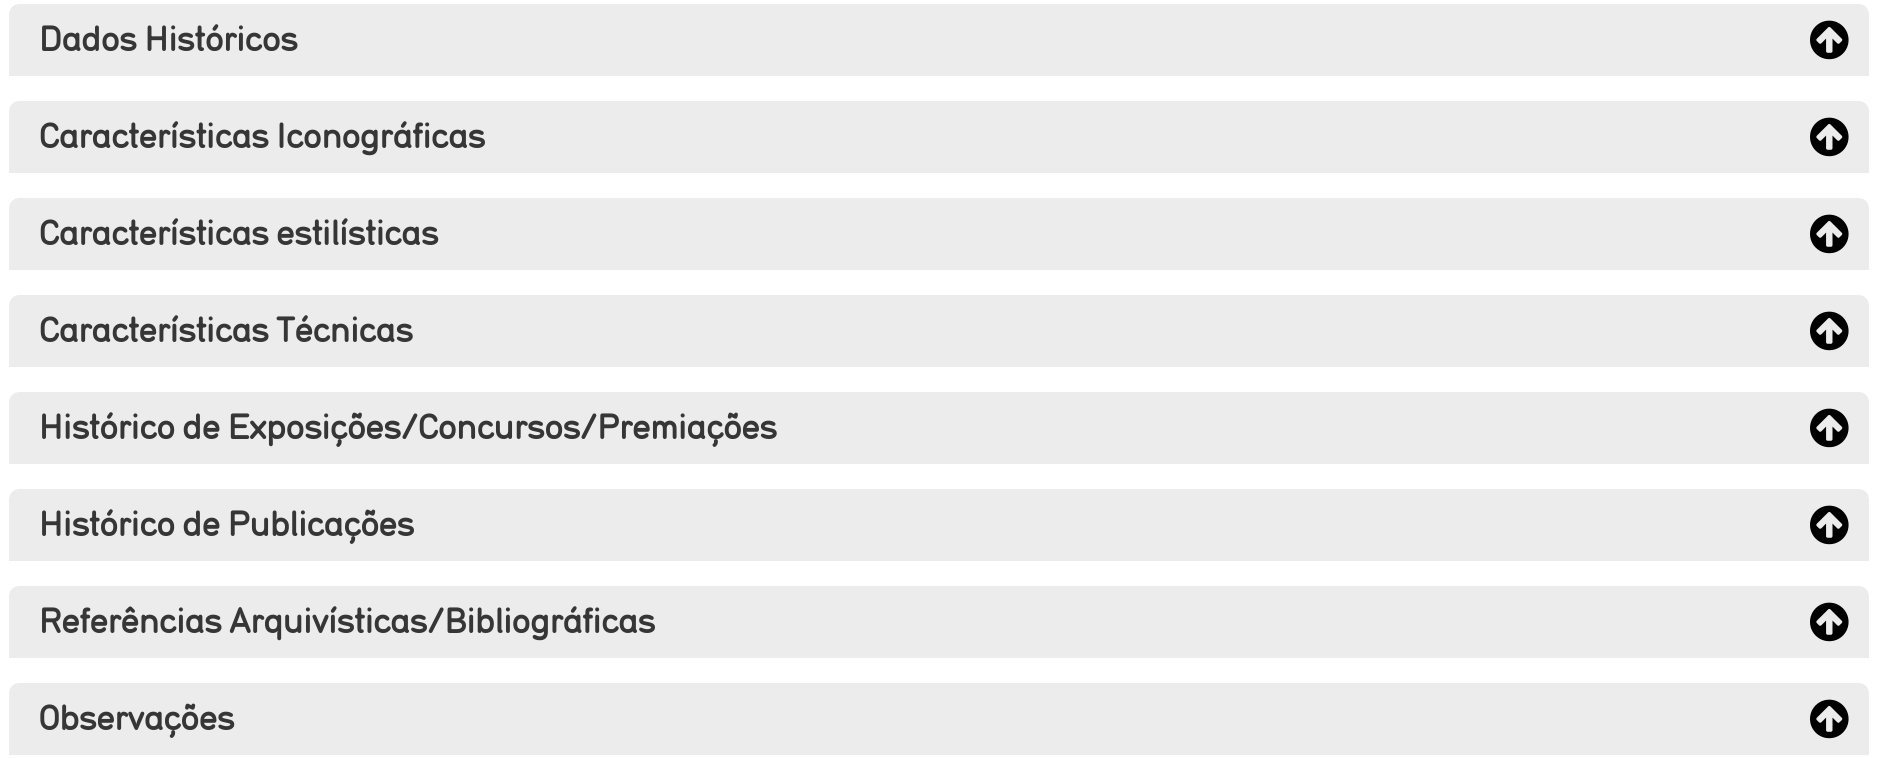
\includegraphics[width=\linewidth]{elementoFichaAnalise}
\end{flushleft}

\subsection{Dados Históricos}
\begin{flushleft}
	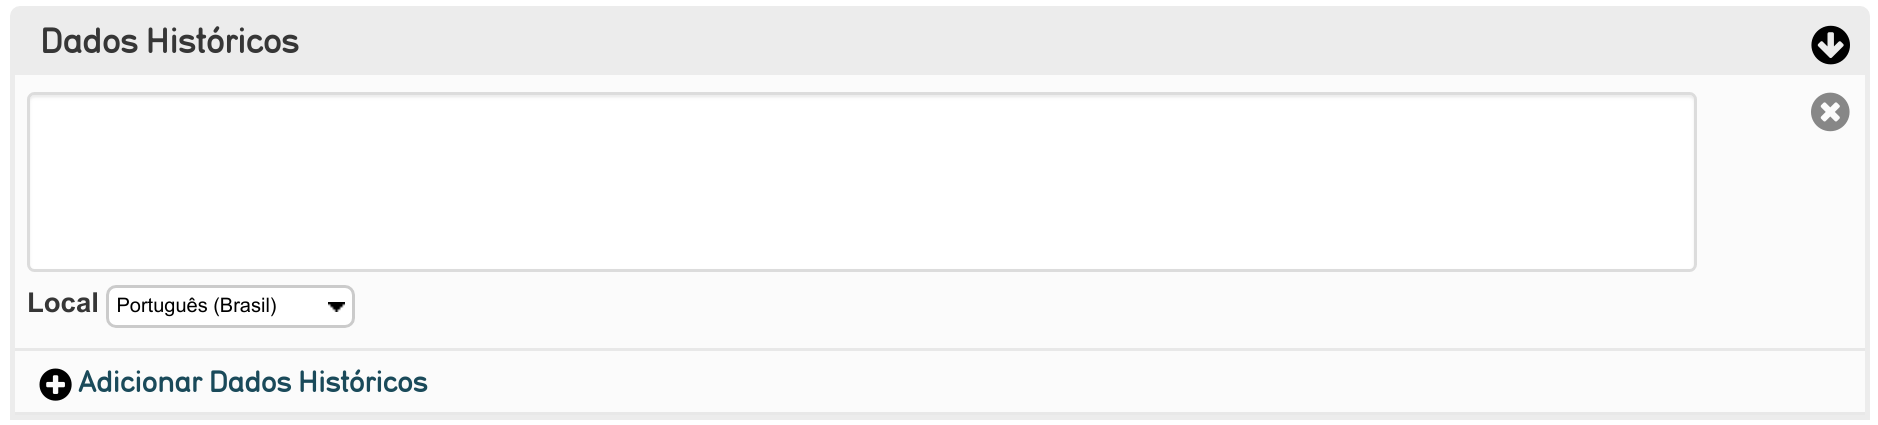
\includegraphics[width=\linewidth]{elemento-18}
\end{flushleft}

\subsection{Características Iconográficas}
\begin{flushleft}
	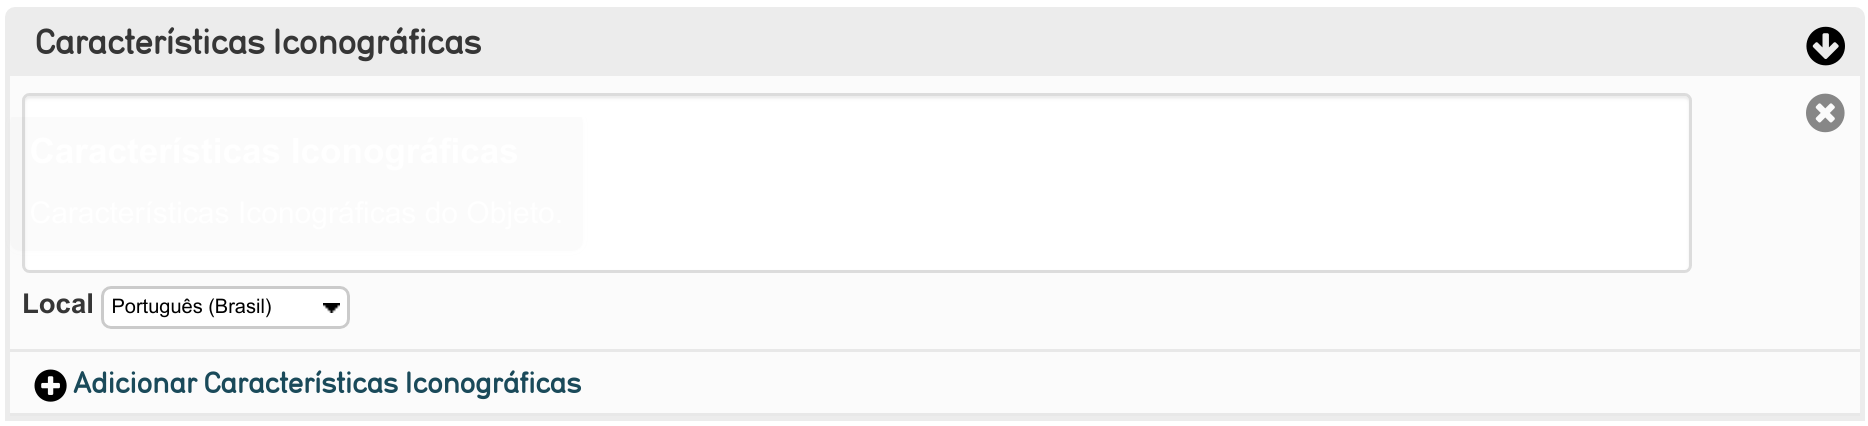
\includegraphics[width=\linewidth]{elemento-19}
\end{flushleft}

\subsection{Características Estilísticas}
\begin{flushleft}
	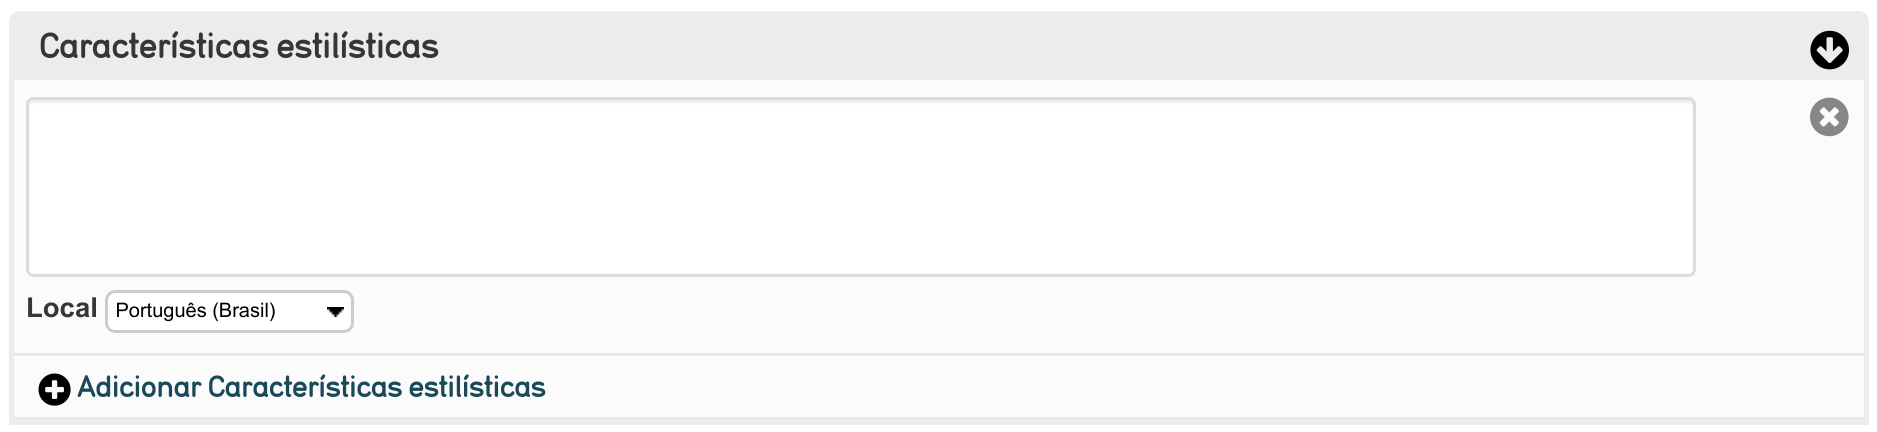
\includegraphics[width=\linewidth]{elemento-20}
\end{flushleft}

\subsection{Características Técnicas}
\begin{flushleft}
	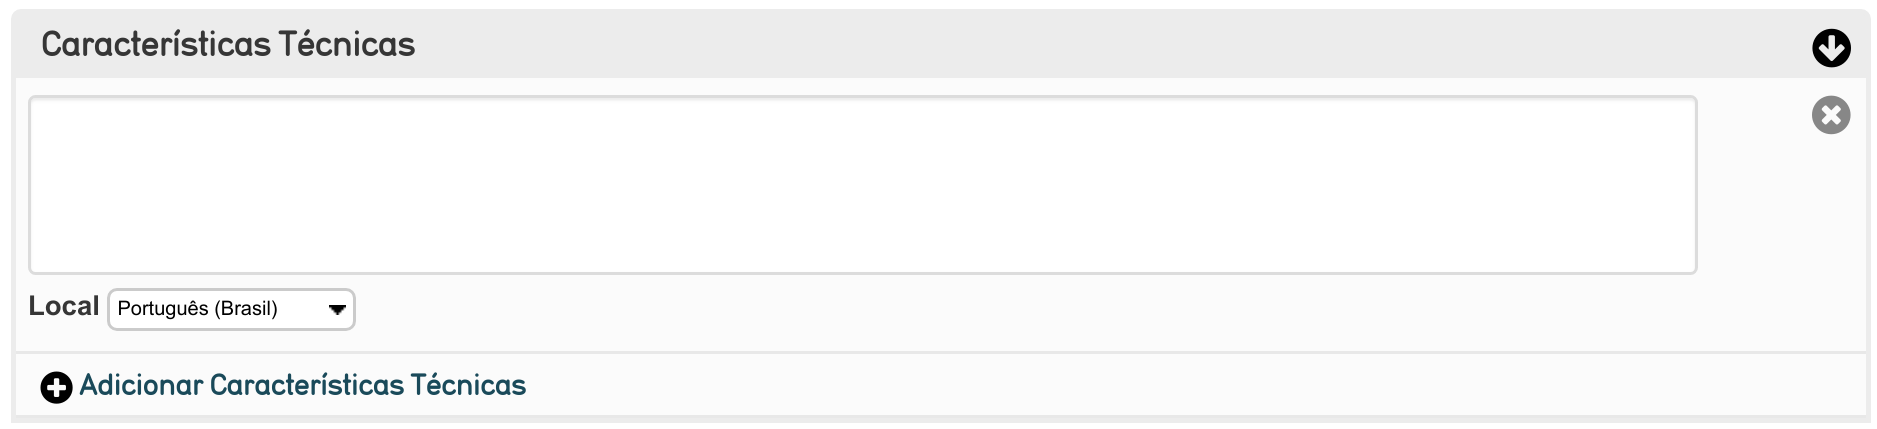
\includegraphics[width=\linewidth]{elemento-21}
\end{flushleft}

\subsection{Histórico de Exposições/Concursos/Premiações}
\begin{flushleft}
	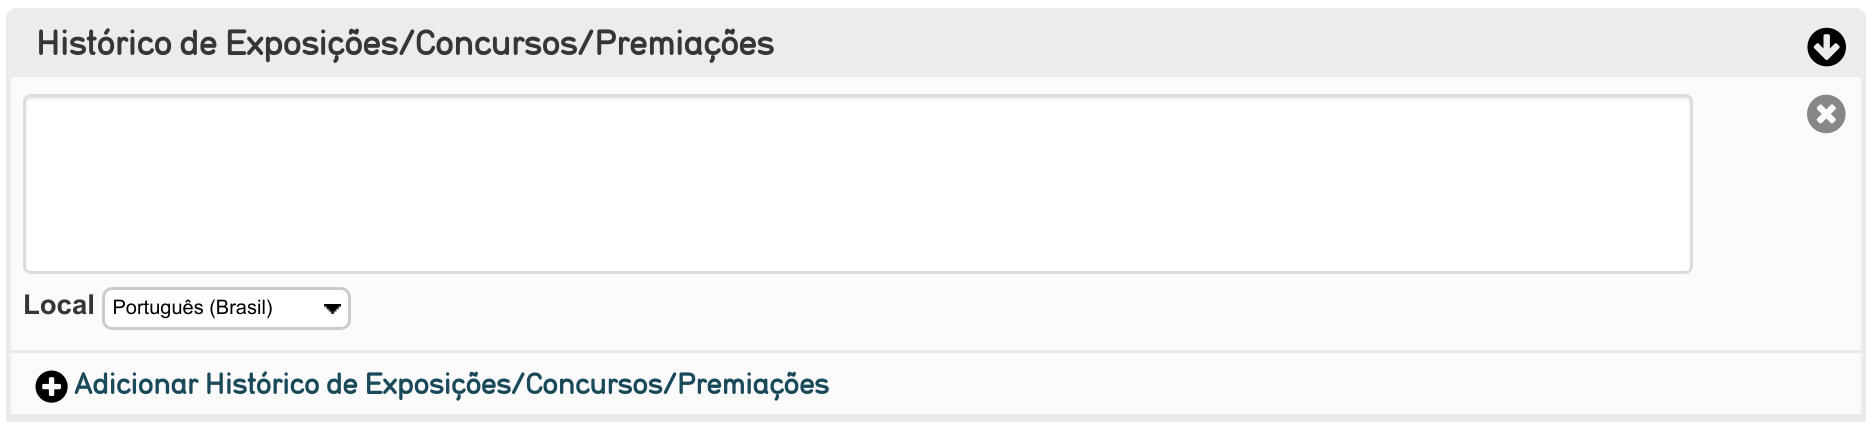
\includegraphics[width=\linewidth]{elemento-22}
\end{flushleft}

\subsection{Histórico de Publicações}
\begin{flushleft}
	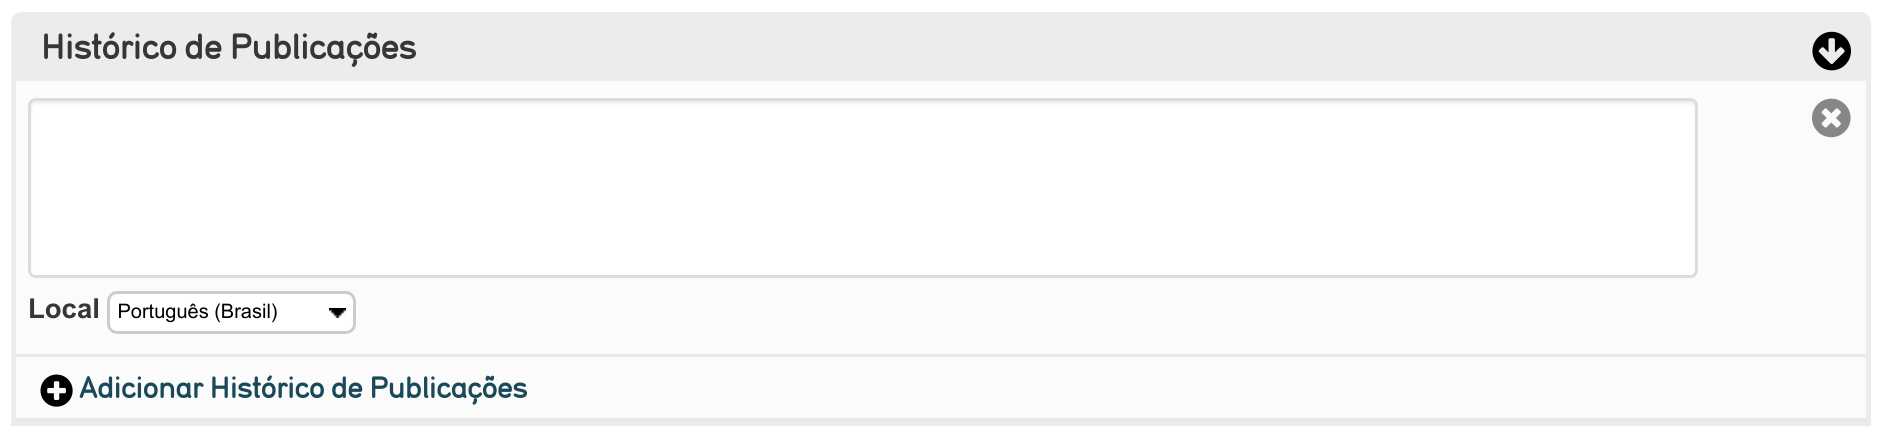
\includegraphics[width=\linewidth]{elemento-23}
\end{flushleft}

\subsection{Referências Arquivísticas/Bibliográficas}
\begin{flushleft}
	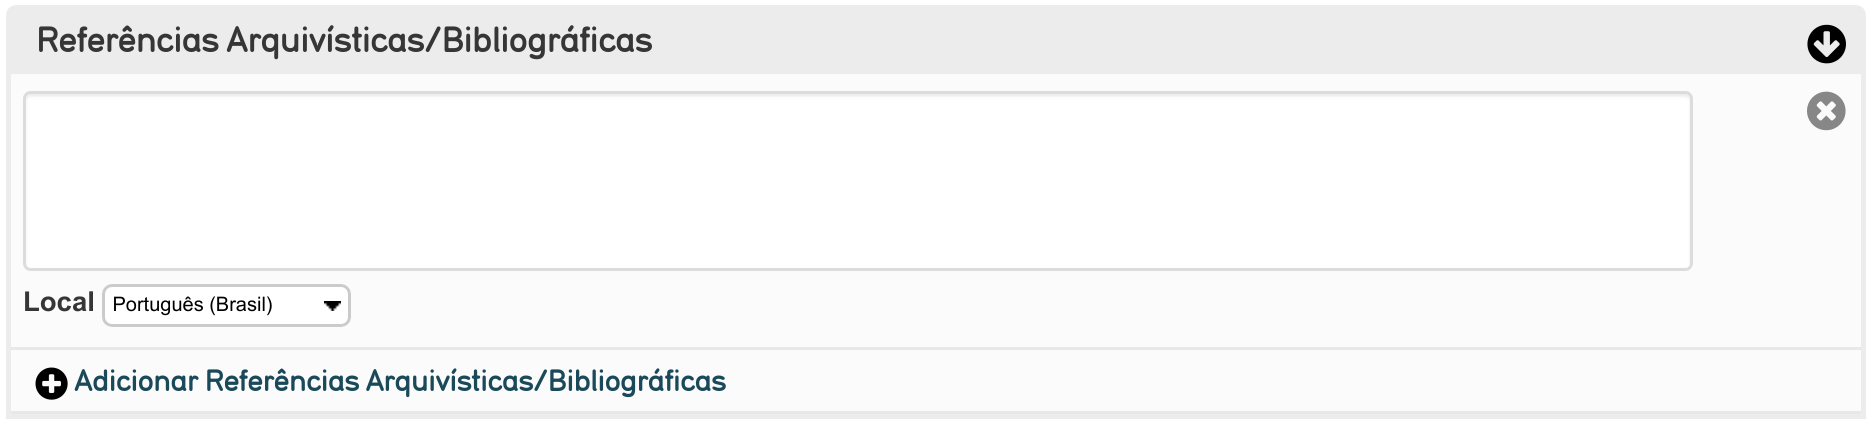
\includegraphics[width=\linewidth]{elemento-24}
\end{flushleft}

\subsection{Observações}
\begin{flushleft}
	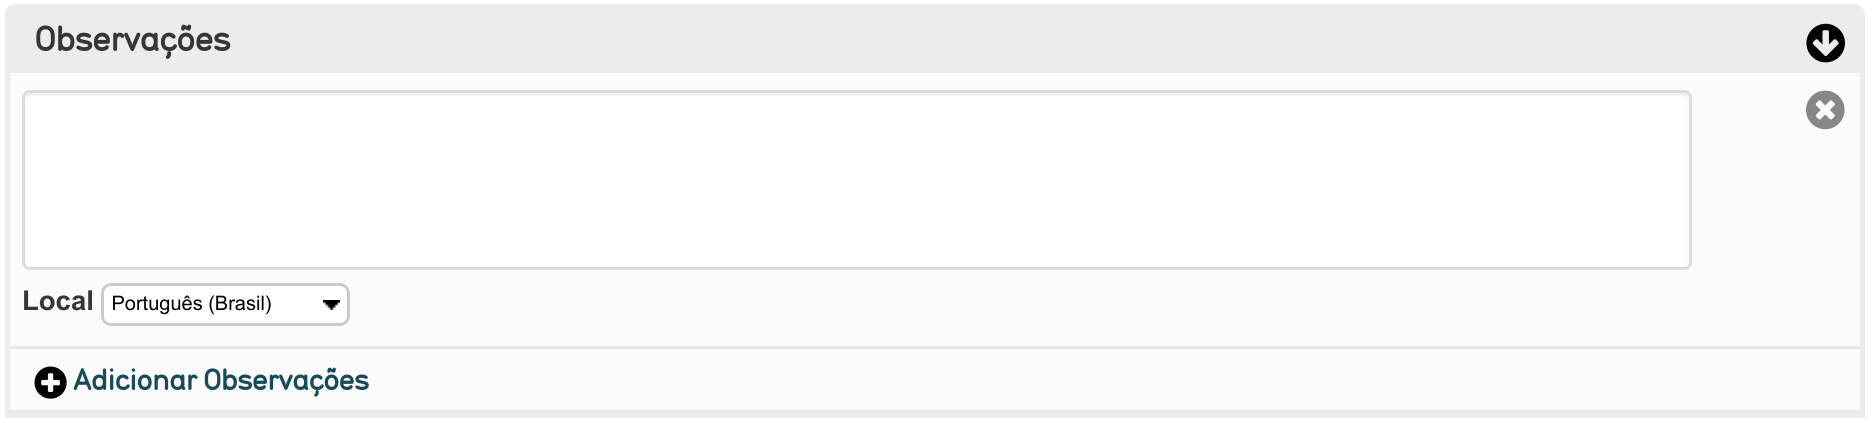
\includegraphics[width=\linewidth]{elemento-25}
\end{flushleft}

\includegraphics{resumo}